% BURST (\method): draft for ICML (Japanese).  Out-of-distribution detection with ONE truncated forward pass of a frozen denoiser and NO training.  Version of 2026-11-26.
%   Two descriptors of the pass (f = unit [channel mean, channel std] of the block U; z = the amplitude profile, one number per block up to the exit block X).
%   The train images are passed once upright and once transposed (rows and columns swapped; the matrix T).  Kept at inference: the upright descriptors and ONE number per
%   train image, the transposition distance tau_g(i) = | g(x_i) - g(T x_i) |.
%       B_g(x) = sum_k w_k log( tau_g(i_k) / r_g(x, i_k) ),  w_k = (1/k) / H_N  (train images sorted by distance),      score = d_f B_f + d_z B_z.
%   Theory (Section 5): Theorem 1 (the response of the ideal denoiser to a transposed input differs by -sigma^2 grad of the log odds "upright against transposed"; zero iff the
%   distribution is symmetric under T), Lemma 1 (the pooled descriptors), Theorem 2 (the pixel permutations that keep adjacency are the eight symmetries of the square),
%   Corollary 2 (one defect per coset), Proposition 1 (when the unit helps).
%   26f WIP, Japanese; MIRU 2025 class.  Image splits: train / val1 / val2 (development) / test (main text) / test' (supplement); server names test2 / testc.
% build: python3 gen/mk.py && latexmk -r latexmkrc main.tex
%   numbers.tex, tab_*.tex, supp_*.tex and the data figures (figs/fig_hist_*, fig_pairs, fig_blk, fig_rho, fig_sym) are written by gen/mk.py from data/*.json.
\documentclass[MIRU,submit]{miru2025j}
\usepackage[dvipdfmx]{graphicx}
\usepackage[dvipdfmx,table]{xcolor}
\definecolor{firstblue}{RGB}{189,215,238}   % cells where Ours ties or beats the comparison value (light blue)
\definecolor{lossred}{RGB}{246,200,192}      % per-pair tables: the comparison value is above Ours (light red)
\definecolor{navyc}{RGB}{31,58,122}\definecolor{redc}{RGB}{192,57,43}\definecolor{markpurple}{RGB}{75,42,123}
\usepackage{amsmath,amssymb}
\usepackage{booktabs}
\usepackage{multirow}
\usepackage{adjustbox}
\usepackage{float}
\usepackage{array}
\usepackage{tikz}
\usetikzlibrary{arrows.meta,positioning,calc,fit,decorations.pathreplacing,shapes.geometric,angles,quotes}
\usepackage{pgfplots}
\pgfplotsset{compat=1.16}
\usepgfplotslibrary{groupplots}
\makeatletter
\renewcommand{\signame}{ICML 2027 投稿原稿のたたき台(日本語)}
\renewcommand{\MIRUPreface}{}
\makeatother
\newcommand{\Tm}{\mathbf{T}}            % the transposition acting on the image (a matrix: bold)
\newcommand{\Hm}{\mathbf{H}}            % a symmetry of the square (or any orthogonal matrix) acting on the image
\newcommand{\Sm}{\mathbf{S}}\newcommand{\Rm}{\mathbf{R}}\renewcommand{\Im}{\mathbf{I}}   % horizontal flip, rotation by 90 degrees, identity
\newcommand{\thm}[2]{\par\vspace{0.6mm}\noindent\textbf{#1}#2\textbf{.}\ }             % a numbered statement: \thm{定理1}{(名前)}
\newcommand{\testp}{test$'$}
\newcommand{\method}{BURST}                 % the name of the method: change it here (and nowhere else)
% the mark beside the name in the title: a square, its main diagonal, and a point with its mirror image (the transposition)
\DeclareRobustCommand{\tramark}{\tikz[baseline=-0.37em, x=1em, y=1em]{\draw[markpurple, line width=0.075em, line join=round] (-0.46,-0.46) rectangle (0.46,0.46);
  \draw[markpurple!60, line width=0.05em, dash pattern=on 0.1em off 0.08em] (-0.46,0.46) -- (0.46,-0.46);
  \fill[markpurple] (0.11,0.27) circle (0.105); \draw[markpurple, fill=white, line width=0.05em] (-0.27,-0.11) circle (0.095);}}
\newcommand{\figlab}{\fontsize{6.2}{7.6}\selectfont}   % the labels inside the hand-drawn figures
\makeatletter\newcommand{\inputrows}[1]{\@@input #1 }\makeatother
\renewcommand{\eqref}[1]{(\ref{#1})}
\renewcommand{\dbltopfraction}{0.95}\renewcommand{\topfraction}{0.95}\renewcommand{\textfraction}{0.05}\renewcommand{\dblfloatpagefraction}{0.78}\setcounter{dbltopnumber}{3}\setcounter{topnumber}{3}
\renewcommand{\floatpagefraction}{0.9}
\makeatletter
\renewenvironment{figure*}{\@floatenv\capwidth\textwidth\ecapwidth\textwidth\abovecaptionskip1mm\belowcaptionskip\z@\@dblfloat{figure}}{\end@dblfloat}
\renewenvironment{table*}{\@floatenv\capwidth\textwidth\ecapwidth\textwidth\abovecaptionskip\z@\belowcaptionskip1mm\@dblfloat{table}}{\end@dblfloat}
\renewenvironment{table}{\@floatenv\capwidth\columnwidth\ecapwidth\columnwidth\abovecaptionskip\z@\belowcaptionskip1mm\@float{table}}{\end@float}
\makeatother
% written by gen/mk.py
\newcommand{\nOursT}{96.5}
\newcommand{\nOursLoT}{96.1}
\newcommand{\nOursHiT}{96.8}
\newcommand{\nUdT}{84.5}
\newcommand{\nHfT}{57.6}
\newcommand{\nFprT}{13.8}
\newcommand{\nPriorT}{88.0}
\newcommand{\nPriorUdT}{73.6}
\newcommand{\nPriorFprT}{35.9}
\newcommand{\nPriorHfT}{56.9}
\newcommand{\nGapPriorT}{8.5}
\newcommand{\nGapPriorLoT}{7.9}
\newcommand{\nGapPriorHiT}{9.1}
\newcommand{\nPriorWinT}{39}
\newcommand{\nPriorTieT}{12}
\newcommand{\nPriorLossT}{0}
\newcommand{\nDiagT}{85.6}
\newcommand{\nDiagUdT}{61.4}
\newcommand{\nDiagFprT}{45.5}
\newcommand{\nDiagHfT}{50.3}
\newcommand{\nGapDiagT}{10.8}
\newcommand{\nGapDiagLoT}{10.1}
\newcommand{\nGapDiagHiT}{11.5}
\newcommand{\nDiagWinT}{43}
\newcommand{\nDiagTieT}{8}
\newcommand{\nDiagLossT}{0}
\newcommand{\nTrainedT}{95.3}
\newcommand{\nTrainedUdT}{93.6}
\newcommand{\nTrainedFprT}{16.9}
\newcommand{\nTrainedHfT}{74.2}
\newcommand{\nGapTrainedT}{1.1}
\newcommand{\nGapTrainedLoT}{0.8}
\newcommand{\nGapTrainedHiT}{1.4}
\newcommand{\nTrainedWinT}{9}
\newcommand{\nTrainedTieT}{31}
\newcommand{\nTrainedLossT}{11}
\newcommand{\nNoUnitT}{93.6}
\newcommand{\nNoUnitUdT}{76.3}
\newcommand{\nNoUnitFprT}{24.1}
\newcommand{\nNoUnitHfT}{55.9}
\newcommand{\nGapNoUnitT}{2.8}
\newcommand{\nGapNoUnitLoT}{2.5}
\newcommand{\nGapNoUnitHiT}{3.2}
\newcommand{\nNoUnitWinT}{26}
\newcommand{\nNoUnitTieT}{24}
\newcommand{\nNoUnitLossT}{1}
\newcommand{\nSevenT}{96.3}
\newcommand{\nSevenUdT}{84.9}
\newcommand{\nSevenFprT}{15.6}
\newcommand{\nSevenHfT}{58.5}
\newcommand{\nGapSevenT}{0.2}
\newcommand{\nGapSevenLoT}{0.1}
\newcommand{\nGapSevenHiT}{0.3}
\newcommand{\nSevenWinT}{19}
\newcommand{\nSevenTieT}{28}
\newcommand{\nSevenLossT}{4}
\newcommand{\nLocalT}{92.9}
\newcommand{\nLocalUdT}{74.9}
\newcommand{\nLocalFprT}{26.4}
\newcommand{\nLocalHfT}{54.8}
\newcommand{\nGapLocalT}{3.6}
\newcommand{\nGapLocalLoT}{3.2}
\newcommand{\nGapLocalHiT}{4.0}
\newcommand{\nLocalWinT}{29}
\newcommand{\nLocalTieT}{20}
\newcommand{\nLocalLossT}{2}
\newcommand{\nLocalHT}{91.2}
\newcommand{\nLocalHUdT}{77.1}
\newcommand{\nLocalHFprT}{26.5}
\newcommand{\nLocalHHfT}{56.3}
\newcommand{\nGapLocalHT}{5.3}
\newcommand{\nGapLocalHLoT}{4.9}
\newcommand{\nGapLocalHHiT}{5.7}
\newcommand{\nLocalHWinT}{29}
\newcommand{\nLocalHTieT}{19}
\newcommand{\nLocalHLossT}{3}
\newcommand{\nUHfT}{89.9}
\newcommand{\nUHfUdT}{75.5}
\newcommand{\nUHfFprT}{35.4}
\newcommand{\nUHfHfT}{56.4}
\newcommand{\nGapUHfT}{6.6}
\newcommand{\nGapUHfLoT}{6.1}
\newcommand{\nGapUHfHiT}{7.1}
\newcommand{\nUHfWinT}{33}
\newcommand{\nUHfTieT}{18}
\newcommand{\nUHfLossT}{0}
\newcommand{\nUVfT}{93.6}
\newcommand{\nUVfUdT}{85.1}
\newcommand{\nUVfFprT}{26.5}
\newcommand{\nUVfHfT}{57.5}
\newcommand{\nGapUVfT}{2.9}
\newcommand{\nGapUVfLoT}{2.5}
\newcommand{\nGapUVfHiT}{3.2}
\newcommand{\nUVfWinT}{22}
\newcommand{\nUVfTieT}{25}
\newcommand{\nUVfLossT}{4}
\newcommand{\nURotT}{95.7}
\newcommand{\nURotUdT}{84.8}
\newcommand{\nURotFprT}{19.4}
\newcommand{\nURotHfT}{57.6}
\newcommand{\nGapURotT}{0.7}
\newcommand{\nGapURotLoT}{0.6}
\newcommand{\nGapURotHiT}{0.9}
\newcommand{\nURotWinT}{22}
\newcommand{\nURotTieT}{26}
\newcommand{\nURotLossT}{3}
\newcommand{\nUCfourT}{96.4}
\newcommand{\nUCfourUdT}{85.0}
\newcommand{\nUCfourFprT}{14.8}
\newcommand{\nUCfourHfT}{58.1}
\newcommand{\nGapUCfourT}{0.1}
\newcommand{\nGapUCfourLoT}{0.1}
\newcommand{\nGapUCfourHiT}{0.2}
\newcommand{\nUCfourWinT}{13}
\newcommand{\nUCfourTieT}{35}
\newcommand{\nUCfourLossT}{3}
\newcommand{\nUSwapT}{96.4}
\newcommand{\nUSwapUdT}{84.6}
\newcommand{\nUSwapFprT}{13.7}
\newcommand{\nUSwapHfT}{57.9}
\newcommand{\nGapUSwapT}{0.0}
\newcommand{\nGapUSwapLoT}{-0.0}
\newcommand{\nGapUSwapHiT}{0.0}
\newcommand{\nUSwapWinT}{5}
\newcommand{\nUSwapTieT}{41}
\newcommand{\nUSwapLossT}{5}
\newcommand{\nOursCtenT}{96.0}
\newcommand{\nTrainedCtenT}{96.4}
\newcommand{\nUdCtenT}{90.7}
\newcommand{\nHfCtenT}{51.4}
\newcommand{\nNoUnitCtenT}{92.8}
\newcommand{\nOursSvhnT}{98.9}
\newcommand{\nTrainedSvhnT}{98.7}
\newcommand{\nUdSvhnT}{58.9}
\newcommand{\nHfSvhnT}{61.5}
\newcommand{\nNoUnitSvhnT}{97.6}
\newcommand{\nOursCelebT}{100.0}
\newcommand{\nTrainedCelebT}{100.0}
\newcommand{\nUdCelebT}{99.9}
\newcommand{\nHfCelebT}{50.2}
\newcommand{\nNoUnitCelebT}{100.0}
\newcommand{\nOursInT}{87.7}
\newcommand{\nTrainedInT}{81.6}
\newcommand{\nUdInT}{77.2}
\newcommand{\nHfInT}{50.3}
\newcommand{\nNoUnitInT}{78.0}
\newcommand{\nOursFmT}{99.7}
\newcommand{\nTrainedFmT}{99.9}
\newcommand{\nUdFmT}{96.0}
\newcommand{\nHfFmT}{74.6}
\newcommand{\nNoUnitFmT}{99.7}
\newcommand{\nOursC}{96.7}
\newcommand{\nOursLoC}{96.4}
\newcommand{\nOursHiC}{97.1}
\newcommand{\nUdC}{85.1}
\newcommand{\nHfC}{57.3}
\newcommand{\nFprC}{11.5}
\newcommand{\nPriorC}{87.9}
\newcommand{\nPriorUdC}{73.8}
\newcommand{\nPriorFprC}{37.8}
\newcommand{\nPriorHfC}{57.3}
\newcommand{\nGapPriorC}{8.8}
\newcommand{\nGapPriorLoC}{8.2}
\newcommand{\nGapPriorHiC}{9.5}
\newcommand{\nPriorWinC}{37}
\newcommand{\nPriorTieC}{14}
\newcommand{\nPriorLossC}{0}
\newcommand{\nDiagC}{85.5}
\newcommand{\nDiagUdC}{61.3}
\newcommand{\nDiagFprC}{44.6}
\newcommand{\nDiagHfC}{50.0}
\newcommand{\nGapDiagC}{11.2}
\newcommand{\nGapDiagLoC}{10.5}
\newcommand{\nGapDiagHiC}{11.9}
\newcommand{\nDiagWinC}{43}
\newcommand{\nDiagTieC}{8}
\newcommand{\nDiagLossC}{0}
\newcommand{\nTrainedC}{95.7}
\newcommand{\nTrainedUdC}{94.1}
\newcommand{\nTrainedFprC}{13.8}
\newcommand{\nTrainedHfC}{74.8}
\newcommand{\nGapTrainedC}{1.0}
\newcommand{\nGapTrainedLoC}{0.7}
\newcommand{\nGapTrainedHiC}{1.3}
\newcommand{\nTrainedWinC}{9}
\newcommand{\nTrainedTieC}{33}
\newcommand{\nTrainedLossC}{9}
\newcommand{\nNoUnitC}{94.0}
\newcommand{\nNoUnitUdC}{77.2}
\newcommand{\nNoUnitFprC}{22.5}
\newcommand{\nNoUnitHfC}{56.1}
\newcommand{\nGapNoUnitC}{2.8}
\newcommand{\nGapNoUnitLoC}{2.4}
\newcommand{\nGapNoUnitHiC}{3.1}
\newcommand{\nNoUnitWinC}{24}
\newcommand{\nNoUnitTieC}{27}
\newcommand{\nNoUnitLossC}{0}
\newcommand{\nSevenC}{96.6}
\newcommand{\nSevenUdC}{85.4}
\newcommand{\nSevenFprC}{13.8}
\newcommand{\nSevenHfC}{58.7}
\newcommand{\nGapSevenC}{0.2}
\newcommand{\nGapSevenLoC}{0.1}
\newcommand{\nGapSevenHiC}{0.3}
\newcommand{\nSevenWinC}{16}
\newcommand{\nSevenTieC}{32}
\newcommand{\nSevenLossC}{3}
\newcommand{\nLocalC}{93.2}
\newcommand{\nLocalUdC}{75.5}
\newcommand{\nLocalFprC}{24.7}
\newcommand{\nLocalHfC}{54.7}
\newcommand{\nGapLocalC}{3.6}
\newcommand{\nGapLocalLoC}{3.2}
\newcommand{\nGapLocalHiC}{3.9}
\newcommand{\nLocalWinC}{30}
\newcommand{\nLocalTieC}{20}
\newcommand{\nLocalLossC}{1}
\newcommand{\nLocalHC}{91.5}
\newcommand{\nLocalHUdC}{77.6}
\newcommand{\nLocalHFprC}{24.7}
\newcommand{\nLocalHHfC}{56.7}
\newcommand{\nGapLocalHC}{5.2}
\newcommand{\nGapLocalHLoC}{4.8}
\newcommand{\nGapLocalHHiC}{5.7}
\newcommand{\nLocalHWinC}{28}
\newcommand{\nLocalHTieC}{22}
\newcommand{\nLocalHLossC}{1}
\newcommand{\nUHfC}{90.2}
\newcommand{\nUHfUdC}{76.2}
\newcommand{\nUHfFprC}{35.1}
\newcommand{\nUHfHfC}{57.1}
\newcommand{\nGapUHfC}{6.5}
\newcommand{\nGapUHfLoC}{5.9}
\newcommand{\nGapUHfHiC}{7.1}
\newcommand{\nUHfWinC}{34}
\newcommand{\nUHfTieC}{17}
\newcommand{\nUHfLossC}{0}
\newcommand{\nUVfC}{93.9}
\newcommand{\nUVfUdC}{85.8}
\newcommand{\nUVfFprC}{24.0}
\newcommand{\nUVfHfC}{57.5}
\newcommand{\nGapUVfC}{2.9}
\newcommand{\nGapUVfLoC}{2.6}
\newcommand{\nGapUVfHiC}{3.2}
\newcommand{\nUVfWinC}{24}
\newcommand{\nUVfTieC}{23}
\newcommand{\nUVfLossC}{4}
\newcommand{\nURotC}{96.0}
\newcommand{\nURotUdC}{85.3}
\newcommand{\nURotFprC}{17.5}
\newcommand{\nURotHfC}{57.7}
\newcommand{\nGapURotC}{0.8}
\newcommand{\nGapURotLoC}{0.6}
\newcommand{\nGapURotHiC}{1.0}
\newcommand{\nURotWinC}{24}
\newcommand{\nURotTieC}{24}
\newcommand{\nURotLossC}{3}
\newcommand{\nUCfourC}{96.6}
\newcommand{\nUCfourUdC}{85.4}
\newcommand{\nUCfourFprC}{12.8}
\newcommand{\nUCfourHfC}{58.1}
\newcommand{\nGapUCfourC}{0.1}
\newcommand{\nGapUCfourLoC}{0.0}
\newcommand{\nGapUCfourHiC}{0.2}
\newcommand{\nUCfourWinC}{7}
\newcommand{\nUCfourTieC}{41}
\newcommand{\nUCfourLossC}{3}
\newcommand{\nUSwapC}{96.7}
\newcommand{\nUSwapUdC}{85.1}
\newcommand{\nUSwapFprC}{11.6}
\newcommand{\nUSwapHfC}{57.7}
\newcommand{\nGapUSwapC}{0.0}
\newcommand{\nGapUSwapLoC}{-0.0}
\newcommand{\nGapUSwapHiC}{0.0}
\newcommand{\nUSwapWinC}{3}
\newcommand{\nUSwapTieC}{42}
\newcommand{\nUSwapLossC}{6}
\newcommand{\nOursCtenC}{97.0}
\newcommand{\nTrainedCtenC}{97.2}
\newcommand{\nUdCtenC}{93.2}
\newcommand{\nHfCtenC}{51.1}
\newcommand{\nNoUnitCtenC}{94.0}
\newcommand{\nOursSvhnC}{99.4}
\newcommand{\nTrainedSvhnC}{99.4}
\newcommand{\nUdSvhnC}{58.2}
\newcommand{\nHfSvhnC}{62.1}
\newcommand{\nNoUnitSvhnC}{97.9}
\newcommand{\nOursCelebC}{100.0}
\newcommand{\nTrainedCelebC}{100.0}
\newcommand{\nUdCelebC}{100.0}
\newcommand{\nHfCelebC}{50.3}
\newcommand{\nNoUnitCelebC}{100.0}
\newcommand{\nOursInC}{87.4}
\newcommand{\nTrainedInC}{82.0}
\newcommand{\nUdInC}{77.1}
\newcommand{\nHfInC}{50.4}
\newcommand{\nNoUnitInC}{78.0}
\newcommand{\nOursFmC}{99.9}
\newcommand{\nTrainedFmC}{100.0}
\newcommand{\nUdFmC}{96.8}
\newcommand{\nHfFmC}{72.4}
\newcommand{\nNoUnitFmC}{99.9}
\newcommand{\nRotT}{88.3}
\newcommand{\nRotUdT}{93.9}
\newcommand{\nEigenUdT}{78.6}
\newcommand{\nPriorFprBestT}{35.9}
\newcommand{\nGepcT}{75.4}
\newcommand{\nPriorBestCtenT}{85.4}
\newcommand{\nPriorBestSvhnT}{99.8}
\newcommand{\nPriorBestCelebT}{99.8}
\newcommand{\nPriorBestInT}{65.5}
\newcommand{\nPriorBestFmT}{99.8}
\newcommand{\nDiffPathSvhnT}{99.8}
\newcommand{\nDiffPathInT}{55.5}
\newcommand{\nNllFmT}{32.8}
\newcommand{\nUVfSvhnT}{86.3}
\newcommand{\nUHfFmT}{87.9}
\newcommand{\nNLossPairs}{11}
\newcommand{\nNLossSvhn}{11}
\newcommand{\nCfsKnnCelebInT}{46.4}
\newcommand{\nPairCHundT}{89.3}
\newcommand{\nPairSsbT}{63.8}
\newcommand{\nPairNincoT}{81.5}
\newcommand{\nPairInatT}{92.9}
\newcommand{\nPassX}{0.54}
\newcommand{\nPassXMin}{0.45}
\newcommand{\nPassXMax}{0.64}
\newcommand{\nAllX}{0.65}
\newcommand{\nAllKnn}{1.01}
\newcommand{\nSearchShareMax}{18}
\newcommand{\nSearchShareMin}{1}
\newcommand{\nDimFMin}{12}
\newcommand{\nDimFMax}{20}
\newcommand{\nDimZMin}{7}
\newcommand{\nDimZMax}{12}
\newcommand{\nNzMin}{11}
\newcommand{\nNzMax}{28}
\newcommand{\nPriorUpT}{40}
\newcommand{\nPriorSameT}{9}
\newcommand{\nPriorDownT}{2}
\newcommand{\nAucTrMin}{76.6}
\newcommand{\nAucTrMax}{100.0}
\newcommand{\nAucTrCten}{90.8}
\newcommand{\nAucHfCten}{53.0}
\newcommand{\nAucTrSvhn}{97.2}
\newcommand{\nAucHfSvhn}{64.7}
\newcommand{\nAucTrCeleb}{100.0}
\newcommand{\nAucHfCeleb}{49.5}
\newcommand{\nAucTrIn}{76.6}
\newcommand{\nAucHfIn}{50.7}
\newcommand{\nAucTrFm}{95.9}
\newcommand{\nAucHfFm}{76.9}
\newcommand{\nAucSwapMin}{76.3}
\newcommand{\nAucKeepSvhnMin}{61.9}
\newcommand{\nAucKeepSvhnMax}{64.7}
\newcommand{\nRhoRows}{36}
\newcommand{\nRhoInMin}{0.77}
\newcommand{\nRhoInMax}{0.95}
\newcommand{\nSwapRatioMin}{0.97}
\newcommand{\nSwapRatioMax}{1.04}
\newcommand{\nSwapRhoMin}{0.54}
\newcommand{\nSwapRhoMax}{0.96}
\newcommand{\nValNoneOne}{92.93}
\newcommand{\nValNoneTwo}{93.38}
\newcommand{\nValTrOne}{93.15}
\newcommand{\nValTrTwo}{96.30}
\newcommand{\nValSevenOne}{93.12}
\newcommand{\nValSevenTwo}{96.14}
\newcommand{\nValHfOne}{90.99}
\newcommand{\nValHfTwo}{90.03}
\newcommand{\nValVfOne}{91.40}
\newcommand{\nValVfTwo}{93.81}
\newcommand{\nValRotOne}{92.65}
\newcommand{\nValRotTwo}{95.65}
\newcommand{\nValShufOne}{92.46}
\newcommand{\nValShufTwo}{92.81}
\newcommand{\nValNnOne}{91.92}
\newcommand{\nValNnTwo}{92.90}
\newcommand{\nValQswapOne}{92.74}
\newcommand{\nValQswapTwo}{95.22}
\newcommand{\nValHshiftOne}{92.31}
\newcommand{\nValHshiftTwo}{94.22}
\newcommand{\nValNegOne}{92.03}
\newcommand{\nValNegTwo}{93.87}
\newcommand{\nValFonlyOne}{92.40}
\newcommand{\nValFonlyTwo}{94.65}
\newcommand{\nValZonlyOne}{92.01}
\newcommand{\nValZonlyTwo}{94.91}
\newcommand{\nValNoDOne}{92.96}
\newcommand{\nValNoDTwo}{96.10}
\newcommand{\nValRoneOne}{91.13}
\newcommand{\nValRoneTwo}{94.01}
\newcommand{\nValRtenOne}{92.72}
\newcommand{\nValRtenTwo}{95.93}
\newcommand{\nValRhundOne}{93.20}
\newcommand{\nValRhundTwo}{96.11}
\newcommand{\nValRthouOne}{93.08}
\newcommand{\nValRthouTwo}{95.80}
\newcommand{\nValExpTwoOneOne}{93.31}
\newcommand{\nValExpTwoOneTwo}{95.89}
\newcommand{\nValExpOneTwoOne}{92.78}
\newcommand{\nValExpOneTwoTwo}{96.17}
\newcommand{\nValUnitOnlyOne}{88.36}
\newcommand{\nValUnitOnlyTwo}{91.07}
\newcommand{\nValNoneFpr}{24.4}
\newcommand{\nValTrFpr}{14.2}
\newcommand{\nValSwapOneMin}{93.08}
\newcommand{\nValSwapOneMax}{93.15}
\newcommand{\nValSwapTwoMin}{96.25}
\newcommand{\nValSwapTwoMax}{96.33}
\newcommand{\nZtTr}{1.35}
\newcommand{\nZA}{2.65}
\newcommand{\nVrTr}{2.01}
\newcommand{\nZtHf}{-0.15}
\newcommand{\nZtShuf}{-0.01}
\newcommand{\nZtNn}{-0.85}
\newcommand{\nCorrNn}{-0.89}
\newcommand{\nCorrTr}{+0.25}
\newcommand{\nBnGapMax}{0.9}
\newcommand{\nColAllOne}{89.11}
\newcommand{\nColAllTwo}{88.22}
\newcommand{\nColCycOne}{89.24}
\newcommand{\nColCycTwo}{88.26}
\newcommand{\nColHueOne}{89.84}
\newcommand{\nColHueTwo}{88.35}
\newcommand{\nColFOne}{80.74}
\newcommand{\nColFTwo}{75.04}
\newcommand{\nColZOne}{88.67}
\newcommand{\nColZTwo}{90.19}
\newcommand{\nValNonPermTwoMin}{79.37}
\newcommand{\nValNonPermTwoMax}{90.02}
\newcommand{\nSymidSwapGainCtenMin}{4.1}
\newcommand{\nSymidSwapGainSvhnMin}{1.9}
\newcommand{\nSymidSwapGainInMin}{8.3}
\newcommand{\nSymidFmDropMin}{0.01}
\newcommand{\nSymidFmDropMax}{0.17}
\newcommand{\nGainFonly}{1.65}
\newcommand{\nValNoneFOne}{90.25}
\newcommand{\nValNoneFTwo}{90.10}
\newcommand{\nValNoneZOne}{91.43}
\newcommand{\nValNoneZTwo}{90.35}
\newcommand{\nValFullTrOne}{93.11}
\newcommand{\nValFullTrTwo}{96.43}
\newcommand{\nValFullNoneOne}{92.92}
\newcommand{\nValFullNoneTwo}{93.65}
\newcommand{\nValFullSevenOne}{93.08}
\newcommand{\nValFullSevenTwo}{96.30}
\newcommand{\nValOwnOne}{90.52}
\newcommand{\nValOwnTwo}{93.74}
\newcommand{\nEqTrMin}{0.067}
\newcommand{\nEqTrMax}{0.196}
\newcommand{\nEqHfMin}{0.044}
\newcommand{\nEqHfMax}{0.091}
\newcommand{\nEqTrHfMin}{1.28}
\newcommand{\nEqTrHfMax}{2.63}
\newcommand{\nEqLowTrHfMin}{1.15}
\newcommand{\nEqLowTrHfMax}{1.57}
\newcommand{\nNSameU}{4}
\newcommand{\nCelebTrAtU}{99.96}
\newcommand{\nCelebTrBest}{99.97}
\newcommand{\nHistInDist}{79.6}
\newcommand{\nHistInOurs}{92.8}
\newcommand{\nHistCtenDist}{79.3}
\newcommand{\nHistCtenOurs}{90.3}
\newcommand{\nSsbLo}{79.7}
\newcommand{\nSsbRef}{62.1}
\newcommand{\nSsbHi}{53.6}
\newcommand{\nInatLo}{86.9}
\newcommand{\nInatRef}{91.7}
\newcommand{\nInatHi}{94.1}

\usepackage{etoolbox}
\makeatletter
\patchcmd{\@makecaption}{\vskip-1.5mm}{\vskip0.3mm}{}{\PackageError{main}{makecaption not patched}{}}
\setlength{\@fptop}{0pt}\setlength{\@fpbot}{0pt plus 1fil}
\makeatother
\hyphenation{FashionMNIST ImageNet EigenScore DiffPath}
\raggedbottom
\makeatletter
% Figure 1 sits in the title block (full width, above the abstract): a double-column float cannot be placed on the first page
\newcommand{\teaserblock}{\vspace{1mm}\noindent\begin{minipage}{\textwidth}\centering
% fig_teaser.tex -- Figure 1 (in the title block, full width): the idea in three panels.
%   (a) the nearest-neighbour distance has no unit: two inputs at the same distance r from their nearest train image
%   (b) one transposition as the unit: the train image and its transposed copy; the distance tau between their descriptors; r measured in units of tau (same geometry as (a))
%   (c) real scores (figs/fig_hist_in64.tex, written by gen/mk.py): ImageNet-64 against iNaturalist, distance only and TRA
% Colours: navy = train images (kept at inference), white square = the transposed copy (used once), red = the input / OOD.
\begingroup
\tikzset{tz/.style={font=\figlab, line cap=round, line join=round}, lab/.style={font=\figlab, inner sep=1pt, align=center},
  tr/.style={circle, fill=navyc, inner sep=0, minimum size=4.2pt}, cp/.style={rectangle, draw=navyc, fill=white, line width=0.6pt, inner sep=0, minimum size=4.0pt},
  inp/.style={star, star points=5, star point ratio=2.2, fill=redc, inner sep=1.2pt}}
\newcommand{\paneltitle}[1]{{\fontsize{7.4}{9}\selectfont\bfseries #1}\\[0.6mm]}
\noindent
\begin{minipage}[t][47mm][t]{35mm}\centering
\paneltitle{(a) 距離には単位がない}
\begin{tikzpicture}[tz]
\useasboundingbox (0,-0.45) rectangle (3.5,3.55);
\coordinate (A) at (0.75,1.85); \coordinate (B) at (2.45,1.85);
\node[tr] at (A) {}; \node[tr] at (B) {};
\draw[black, line width=0.6pt] (A) -- node[pos=0.5, above left, inner sep=0.6pt, lab] {$r$} ($(A)+(40:0.55)$);
\draw[black, line width=0.6pt] (B) -- node[pos=0.5, above left, inner sep=0.6pt, lab] {$r$} ($(B)+(40:0.55)$);
\node[inp] at ($(A)+(40:0.55)$) {}; \node[inp] at ($(B)+(40:0.55)$) {};
\node[lab, text=navyc] at ($(A)+(0,-0.3)$) {$x_i$}; \node[lab, text=navyc] at ($(B)+(0,-0.3)$) {$x_j$};
\node[lab] at (1.75,0.75) {同じ距離 $r$.\\[1pt]近いのか, 遠いのか?};
\node[tr] at (0.3,0.05) {}; \node[lab, anchor=west] at (0.42,0.05) {train 画像};
\node[inp, inner sep=0.95pt] at (2.0,0.05) {}; \node[lab, anchor=west] at (2.12,0.05) {入力};
\end{tikzpicture}
\end{minipage}\hfill
\begin{minipage}[t][47mm][t]{66mm}\centering
\paneltitle{(b) 転置1つを長さの単位にする}
\begin{tikzpicture}[tz, >={Stealth[length=1.5mm, width=1.2mm]}]
\useasboundingbox (0,-0.45) rectangle (6.6,3.55);
% the train image and its transposed copy
\node[inner sep=0, anchor=south west, draw=navyc, line width=1pt] (im0) at (0.75,2.62) {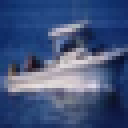
\includegraphics[width=0.78cm]{figs/o0.png}};
\node[inner sep=0, anchor=south west, draw=black!55, line width=0.5pt] (im1) at (2.55,2.62) {
\includegraphics[width=0.78cm]{figs/o5.png}};
\draw[black!45, densely dashed, line width=0.4pt] (im0.north west) -- (im0.south east);
\draw[->, black, line width=0.6pt] (im0.east) -- node[above, lab, inner sep=1.5pt] {転置} (im1.west);
\node[lab, anchor=east, text=navyc] at (0.68,3.01) {$x_i$};
\node[lab, anchor=west, align=left] at (3.5,3.01) {$\mathbf{T}x_i$：縦と横を入れ替える.\\記述子が $\tau$ だけ動く.};
% left: a large transposition distance, the input closer than tau
\coordinate (A) at (1.55,1.25);
\draw[navyc!55, densely dashed, line width=0.5pt] (A) circle (0.9);
\draw[navyc, line width=0.7pt] (A) -- node[pos=0.5, below, inner sep=1.8pt, lab, text=navyc] {$\tau$} ($(A)+(200:0.9)$);
\node[cp] at ($(A)+(200:0.9)$) {}; \node[tr] at (A) {};
\draw[black, line width=0.6pt] (A) -- node[pos=0.5, above left, inner sep=0.6pt, lab] {$r$} ($(A)+(40:0.55)$);
\node[inp] at ($(A)+(40:0.55)$) {};
\node[lab] at (1.55,-0.12) {$\tau/r>1$：分布内らしい};
% right: a small transposition distance, the input farther than tau
\coordinate (B) at (4.75,1.25);
\draw[navyc!55, densely dashed, line width=0.5pt] (B) circle (0.27);
\draw[navyc, line width=0.7pt] (B) -- ($(B)+(200:0.27)$);
\node[cp] at ($(B)+(200:0.27)$) {}; \node[tr] at (B) {};
\draw[black, line width=0.6pt] (B) -- ($(B)+(40:0.55)$);
\node[lab] at ($(B)+(64:0.66)$) {$r$};
\node[inp] at ($(B)+(40:0.55)$) {};
\node[lab, text=navyc] at ($(B)+(-0.42,-0.38)$) {$\tau$};
\node[lab] at (4.75,-0.12) {$\tau/r<1$：分布外らしい};
\node[cp] at (2.74,0.62) {}; \node[lab, anchor=west] at (2.86,0.62) {転置した train 画像};
\draw[navyc!55, densely dashed, line width=0.5pt] (2.62,0.3) -- (2.88,0.3); \node[lab, anchor=west] at (2.92,0.3) {半径 $\tau$};
\end{tikzpicture}
\end{minipage}\hfill
\begin{minipage}[t][47mm][t]{70mm}\centering
\paneltitle{(c) ImageNet-64 と iNaturalist のスコアの分布}
\vspace{0.5mm}
% written by gen/mk.py from data/fig_tra.json (stored test scores, noise seed 0)
\begin{tikzpicture}
\begin{groupplot}[group style={group size=2 by 1, horizontal sep=7mm}, width=38mm, height=33mm,
  tick label style={font=\figlab}, label style={font=\figlab}, title style={font=\figlab, yshift=-1.6mm, align=center}, xlabel={標準化したスコア},
  legend style={font=\figlab, draw=none, fill=none, legend columns=2, /tikz/every even column/.append style={column sep=3mm}}]
\nextgroupplot[title={距離のみ\\AUROC 79.6\%}, ylabel={密度}, legend to name=histlegA]
\addplot[const plot, navyc, line width=0.7pt] coordinates {(-7.50,0.0000) (-7.00,0.0040) (-6.50,0.0040) (-6.00,0.0000) (-5.50,0.0000) (-5.00,0.0000) (-4.50,0.0000) (-4.00,0.0040) (-3.50,0.0120) (-3.00,0.0320) (-2.50,0.0360) (-2.00,0.0440) (-1.50,0.1240) (-1.00,0.1880) (-0.50,0.3920) (0.00,0.5120) (0.50,0.4040) (1.00,0.2160) (1.50,0.0280) (2.00,0.0000) (2.50,0)};
\addplot[const plot, redc, densely dashed, line width=0.7pt] coordinates {(-7.50,0.0000) (-7.00,0.0000) (-6.50,0.0000) (-6.00,0.0200) (-5.50,0.0240) (-5.00,0.0200) (-4.50,0.0560) (-4.00,0.0800) (-3.50,0.0840) (-3.00,0.1520) (-2.50,0.1720) (-2.00,0.2600) (-1.50,0.1760) (-1.00,0.3480) (-0.50,0.2360) (0.00,0.2600) (0.50,0.0960) (1.00,0.0160) (1.50,0.0000) (2.00,0.0000) (2.50,0)};
\legend{分布内の画像, 分布外の画像}
\nextgroupplot[title={\method\\AUROC 92.8\%}]
\addplot[const plot, navyc, line width=0.7pt] coordinates {(-4.50,0.0000) (-4.00,0.0000) (-3.50,0.0080) (-3.00,0.0040) (-2.50,0.0520) (-2.00,0.0600) (-1.50,0.2120) (-1.00,0.3120) (-0.50,0.3360) (0.00,0.3680) (0.50,0.2640) (1.00,0.2840) (1.50,0.1000) (2.00,0.0000) (2.50,0)};
\addplot[const plot, redc, densely dashed, line width=0.7pt] coordinates {(-4.50,0.0000) (-4.00,0.0040) (-3.50,0.0520) (-3.00,0.2400) (-2.50,0.4680) (-2.00,0.5800) (-1.50,0.4480) (-1.00,0.1440) (-0.50,0.0520) (0.00,0.0080) (0.50,0.0040) (1.00,0.0000) (1.50,0.0000) (2.00,0.0000) (2.50,0)};
\end{groupplot}
\end{tikzpicture}\\[-0.5mm]
\pgfplotslegendfromname{histlegA}

\end{minipage}
\endgroup
\par\vspace{0.5mm}
\def\@captype{figure}\capwidth\textwidth\ecapwidth\textwidth\abovecaptionskip1mm\belowcaptionskip\z@
\caption{\textbf{転置1つが, 距離の単位になる.} (a) 最近傍の距離 $r$ には基準になる長さがない. 左右の入力(赤い星)は, train 画像(紺の丸)から同じ距離にある. (b) \method{} は, train 画像と, その縦と横を入れ替えた画像(転置. 白い四角)をノイズ除去器に通し, 2つの記述子の距離 $\tau$ を train 画像ごとに1つの数として持つ. 入力までの距離 $r$ を $\tau$ で割ると, 同じ距離でも, $\tau$ より近ければ分布内らしく, 遠ければ分布外らしい. (c) ImageNet-64 を分布内, iNaturalist を分布外とするときのスコアの分布(test 画像, ノイズの種0). 距離だけでは AUROC が\nHistInDist\%, $\tau$ で割ると\nHistInOurs\%になる.}
\label{fig:teaser}
\end{minipage}\vspace{4mm}}
\let\tra@maketitle\@maketitle
\def\@maketitle{\tra@maketitle\teaserblock}
\makeatother
\begin{document}
\title{\textbf{\tramark\hspace{0.25em}\method：破れた対称性1つを長さの単位にする,\\学習のいらない拡散モデルの分布外検知}}
\affiliate{sfc}{慶應義塾大学 総合政策学部B3 中澤・大越研究室 d-hacks}
\affiliate{sfc2}{慶應義塾大学大学院 政策・メディア研究科}
\author{omote}{}{sfc}[]
\author{親:zackeyさん}{}{sfc2}[]
\maketitle

\section*{概要}
拡散モデルによる分布外検知は, 1枚の画像に10回以上のネットワークの評価を要するか, 分布内データセットによって大きく崩れる. 1回の順伝播で読める中間特徴の最近傍の距離は有望だが, 距離には基準になる長さがない. 本論文は, この長さを, 分布が破っている対称性から得る. 理想的なノイズ除去器では, 対称変換に対する同変性からのずれが, 分布とそれを変換した分布の対数密度比の勾配に等しく, 分布がその変換で変わらないときに限って消えることを示す. 提案する \method{} は, 学習用の画像(train 画像)とその転置(縦と横の入れ替え)の記述子の距離を train 画像ごとに1つの数として持ち, 入力から train 画像までの距離をその数で割る. 学習するパラメータも, 選ぶ近傍数もなく, 推論は途中で打ち切る1回の順伝播で済む. 5つの分布内データセットの51組で, 平均 AUROC は\nOursT\%, FPR95 は\nFprT\%であり, 同じ拡散モデルを用いる10の先行手法の最良(\nPriorT\%, \nPriorFprBestT\%)を上回る. 分布が保つ対称性, 色の対称性, 対称変換でない変換から作った単位は精度を下げ, 効くのは破れた対称性だけである.

\section{はじめに}
学習時に見ていない種類の入力を見分ける分布外検知は, 機械学習のモデルを開いた環境で使うための前提である. 外部のデータで学習した基盤モデル~\cite{oquab2024dinov2,radford2021clip}を前提にできない領域では, 対象の領域のラベルのない画像で学習した生成モデル1つで検知まで完結できることが望ましい. 拡散モデル~\cite{song2021score,karras2022edm}は, そのための有力な候補である.

しかし, 現状の方法には2つの弱点がある. 第1に, 尤度や, 生成の軌跡, スコアの統計量による方法~\cite{nalisnick2019deep,serra2020input,mahmood2021msma,heng2024diffpath,alexis2026gepc,shoushtari2026eigenscore}は, 1枚に10回から数百回のネットワークの評価を要し, 分布内データセットによって大きく崩れる. 第2に, 1回の順伝播で済む方法, すなわちノイズ除去器の中間特徴~\cite{xiang2023ddae}と train 画像との近さを測る方法~\cite{rouzoumka2026cfs}は, 距離に基準になる長さを持たない. 同じ距離が近いのか遠いのかは, 特徴空間の場所によって変わる(図~\ref{fig:teaser}a). しかも, 尤度で知られている逆転~\cite{nalisnick2019deep}が特徴の距離でも起こり, 単純な分布外の画像が分布内の画像より train 画像に近くなる(ImageNet-64 に対する CelebA で, CFS の kNN ヘッドの AUROC は\nCfsKnnCelebInT\%). 距離を近傍の train 画像どうしの距離で割る方法~\cite{breunig2000lof,zelnik2004self}は, その長さ自体が密度から決まるので, 密度の情報を消してしまう(\ref{sec:local}節). そこで, 次の問いを立てる.

\begin{quote}
\textit{密度とは別のところから来る「長さの単位」を, 学習も, 分布外の画像も使わずに, 分布内の画像だけから得られるか.}
\end{quote}

本論文は, この問いに肯定的に答える. 鍵は, \textbf{分布が破っている対称性}である. 画像の縦と横を入れ替える転置は, 画素を並べ替えるだけで, 画素の値も, 隣り合う画素の関係も, 加えるノイズの分布も変えない. 自然画像には縦と横の区別があるので, 転置した train 画像は「内容は分布内と同じで, 分布内ではない画像」になる. train 画像とその転置をノイズ除去器に通したときの記述子の距離は, その train 画像のまわりで, 分布内と分布の外がどれだけ離れているかを教える.

この距離が何を測っているかは, 理論から分かる. 一言でいえば, \textbf{ノイズ除去器は, 分布が破った対称性だけを破る}. 理想的なノイズ除去器の, 転置した入力に対する応答のずれは, 入力が正立の分布と転置した分布のどちらから来たらしいかを表す対数オッズの勾配に比例し(定理1), 分布が転置で変わらなければ消える(系1). 単位に使える変換は正方形の8つの対称変換に限られ(定理2), 転置は, その中で, 調べた5つの分布内のどれでも分布が破っている変換である.

提案する \method{} は, 転置による記述子の動きを長さの単位にする(図~\ref{fig:teaser}b). train 画像とその転置の記述子の距離(転置距離)を train 画像ごとに1つの数として持ち, 入力から train 画像までの距離をその数で割って, 比の対数を, 近い train 画像から順に順位の逆数の重みで平均する. 調整する重みも, 選ぶ近傍数も, 学習するパラメータもなく, 順伝播は記述子を読み終えたブロックで打ち切る.

5つの分布内データセットの51組で, 自然画像の分布外集合での平均 AUROC は\nOursT\%であり, 同じ拡散モデルを用いる先行研究の最良(CFS の kNN ヘッド, \nPriorT\%)を\nGapPriorT{}ポイント上回る(図~\ref{fig:teaser}c に1組の例). FPR95 は\nPriorFprBestT\%から\nFprT\%に下がる. 単位を除くと\nNoUnitT\%に戻る. 本論文の貢献は次の3つである.
\begin{itemize}
\setlength{\itemsep}{0pt}\setlength{\parskip}{0pt}
\item \textbf{手法.} 転置による記述子の動きを長さの単位にする, 学習のない最近傍のスコア(\ref{sec:method}節). 推論は途中で打ち切る1回の順伝播である.
\item \textbf{理論.} 理想的なノイズ除去器の同変性からのずれが, 分布とその変換の対数密度比の勾配に等しいこと, 単位に使える変換が正方形の8つの対称変換に限られること, 単位が精度を上げる条件(\ref{sec:theory}節).
\item \textbf{実験.} 51組で, 同じ拡散モデルを用いる10の先行手法との比較と, 単位を作る変換を替える対照実験(分布が保つ対称性, 色の対称性, 対称変換でない変換, 入れ替えた単位)を行い, 効くのが破れた対称性だけであることを示す(\ref{sec:exp}節).
\end{itemize}


\section{準備}
\label{sec:prep}
\textbf{問題設定.} 分布内の画像の密度を $p(x)$ とし, そこから得られた $N$ 枚の train 画像 $x_1,\ldots,x_N$ が与えられる. 入力画像 $x$ に分布内らしさを表すスコア $s(x)$ を与え, しきい値より小さい入力を分布外と判定する. 評価の指標は AUROC であり, 分布内の画像の95\%を残すときに分布外の画像が通過する割合(FPR95)も示す.

\textbf{ノイズ除去器の中間特徴.} 拡散モデルのノイズ除去器は, ノイズを加えた画像から元の画像を推定するネットワークであり, 多くは, エンコーダで解像度を下げてデコーダで上げる U-Net~\cite{ronneberger2015unet}である. 入力側から数えて $h$ 番目のブロックの出力(特徴マップ)の, チャネル $c$, 位置 $(i,j)$ の値を $h_{c,i,j}$ と書く. 画像 $x$ に小さなノイズ $\sigma_1\varepsilon$ ($\sigma_1=0.01$. $\varepsilon$ はすべての画像に共通の1枚)を加えて, ノイズ除去器に1回通す.

\textbf{最近傍の距離と密度.} 入力の記述子から, $N$ 個の train 画像の記述子のうち $k$ 番目に近いものまでの距離を $r_{(k)}(x)$ とする. 記述子が $d$ 次元の広がりをもつとき, 半径 $r_{(k)}(x)$ の球の体積は $V r_{(k)}(x)^{d}$ ($V$ は半径1の球の体積)である. 球の中で密度が一定とみなせるなら
\begin{equation}
k=N\,p(x)\,V\,r_{(k)}(x)^{d}
\label{eq:knn}
\end{equation}
が成り立つ~\cite{loftsgaarden1965knn}.

\textbf{転置.} 正方形の画像の, 行 $i$, 列 $j$ の画素を, 行 $j$, 列 $i$ に移す変換を転置という. 縦と横を入れ替える変換である. 画素の並べ替えなので, 行列 $\Tm$ を用いて $x\mapsto\Tm x$ と書ける. 転置を2回行うと元に戻る($\Tm\Tm x=x$)ので, $\Tm$ の逆行列は $\Tm$ 自身である.

\section{提案手法：\method}
\label{sec:method}
\begin{figure*}[t]\centering
\begin{adjustbox}{max width=\textwidth}% fig_method.tex -- the method in pictures (TikZ, drawn by hand; absolute coordinates in cm, natural width 17.6 cm = \textwidth).
%   (a) test time: one forward pass of the frozen denoiser, stopped at block X; two descriptors: f (mean and std of the block U)
%       and z (one number per block up to X: the comb under the blocks).
%   (b) once, before: the train images upright and transposed: the upright descriptor is kept, the transposed one gives
%       one number per train image, the transposition distance tau.
%   (c) per descriptor: the distance r to a train image is measured in units of its transposition distance.
%   Colours: black, navy (U, f, train images), red (X, z, the input in panel c).  Schematic.
\providecommand{\figlab}{\fontsize{6.2}{7.6}\selectfont}
\begin{tikzpicture}[font=\figlab, >={Stealth[length=1.6mm, width=1.3mm]}, line join=round, line cap=round,
  lab/.style={font=\figlab, inner sep=1pt, align=center}, ttl/.style={font=\scriptsize, anchor=south west, inner sep=0pt}]
%% ================================================================ (a) test time
\node[ttl] at (0,0.15) {\textbf{(a)}\ テスト時：1回の順伝播を途中で打ち切り, 2つの記述子を読む};
\node[inner sep=0, draw=black, line width=0.6pt] (img) at (0.6,-1.55) {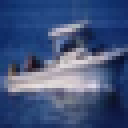
\includegraphics[width=1.05cm]{figs/o0.png}};
\node[lab, anchor=north] at (0.6,-2.16) {入力画像 $x$};
\draw[->] (1.2,-1.55) -- node[above, lab] {$+\sigma_1\varepsilon$} (1.87,-1.55);
% the blocks of the denoiser, left edge / height: encoder (32, 32, 16, 16, 8, 8), decoder (8, U at 8, 16, X at 16), then two blocks at 32
% that are not computed.  One red tick per block up to X: one number per block (the amplitude), collected on the red line.
\def\ybus{-2.68}
\foreach \xl/\h in {1.95/1.8, 2.22/1.8, 2.57/1.25, 2.84/1.25, 3.19/0.78, 3.46/0.78, 3.81/0.78, 4.08/0.78, 4.43/1.25, 4.70/1.25}{
  \draw[redc, line width=0.5pt] ({\xl+0.1},{-1.55-\h/2}) -- ({\xl+0.1},\ybus);
  \fill[redc] ({\xl+0.1},\ybus) circle (0.035);}
\foreach \xl/\h in {1.95/1.8, 2.22/1.8, 2.57/1.25, 2.84/1.25, 3.19/0.78, 3.46/0.78, 3.81/0.78, 4.43/1.25}
  \draw[black, fill=white, line width=0.7pt] (\xl,{-1.55-\h/2}) rectangle ++(0.2,\h);
\draw[navyc, fill=navyc!35, line width=0.9pt] (4.08,-1.94) rectangle ++(0.2,0.78);
\draw[redc, fill=redc!25, line width=0.9pt] (4.70,-2.175) rectangle ++(0.2,1.25);
\foreach \xl in {5.05, 5.32}
  \draw[black!45, densely dashed, line width=0.5pt] (\xl,-2.45) rectangle ++(0.2,1.8);
\draw[redc, line width=0.5pt] (2.05,\ybus) -- (4.80,\ybus);
\node[lab, anchor=south] at (2.8,-0.6) {エンコーダ};
\node[lab, anchor=south west] at (4.34,-0.6) {デコーダ};
\node[lab, anchor=south east, text=navyc] at (4.15,-1.15) {\textbf{U}};
\node[lab, anchor=south, text=redc] at (4.80,-0.92) {\textbf{X}};
\node[lab, anchor=north west, text=black!60] at (4.98,-2.5) {計算しない};
\node[lab, anchor=north west, align=left] at (0.0,-2.98) {凍結したノイズ除去器\\\textcolor{navyc}{\textbf{U}}：読み出しブロック\\\textcolor{redc}{\textbf{X}}：打ち切りブロック};
% the two descriptors
\node[draw=navyc, rounded corners=2pt, line width=0.8pt, inner sep=3pt, align=left, font=\figlab, text width=21mm, anchor=north west] (fbox) at (6.1,-0.45)
  {$f$：U の出力の,\\チャネルごとの\\平均と標準偏差};
\node[draw=redc, rounded corners=2pt, line width=0.8pt, inner sep=3pt, align=left, font=\figlab, text width=21mm, anchor=north west] (zbox) at (6.1,-2.92)
  {$z$：X までの\\各ブロックの出力から\\数値を1つずつ};
\draw[->, navyc, line width=0.7pt] (4.18,-1.16) -- (4.18,-0.12) -- (7.2,-0.12) -- (7.2,-0.45);
\draw[->, redc, line width=0.7pt] (3.425,\ybus) -- (3.425,-3.43) -- (6.1,-3.43);
%% ================================================================ (b) the bank
\node[ttl] at (8.75,0.15) {\textbf{(b)}\ 事前：正立と転置の2通り};
\draw[black!45, rounded corners=3pt] (8.75,-0.15) rectangle (12.25,-4.38);
\node[inner sep=0, draw=navyc, line width=1.5pt] (b0) at (9.55,-1.0) {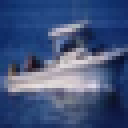
\includegraphics[width=1.05cm]{figs/o0.png}};
\node[inner sep=0, draw=black!55, line width=0.5pt] (b1) at (11.45,-1.0) {
\includegraphics[width=1.05cm]{figs/o5.png}};
\draw[black!45, densely dashed, line width=0.4pt] (b0.north west) -- (b0.south east);
\draw[->, black, line width=0.6pt] (b0.east) -- node[above, lab, inner sep=1.5pt] {転置} (b1.west);
\node[lab, anchor=north, text=navyc] at (9.55,-1.6) {$x_i$}; \node[lab, anchor=north] at (11.45,-1.6) {$\mathbf{T}x_i$};
\draw[navyc, line width=1.0pt] (8.98,-2.46) rectangle ++(0.15,0.15);
\node[lab, anchor=west, align=left, text=navyc] at (9.2,-2.52) {そのまま(正立)の $N$ 枚\\→ バンク(推論時に持つ)};
\draw[black!55, line width=0.6pt] (8.98,-3.2) rectangle ++(0.15,0.15);
\node[lab, anchor=west, align=left, text=black!75] at (9.2,-3.26) {転置した1枚までの距離\\→ 転置距離 $\tau$(1つの数)};
\node[lab, anchor=west, text=black!60] at (8.95,-4.03) {ノイズ $\varepsilon$ は転置しない};
%% ================================================================ (c) the score
\node[ttl] at (12.55,0.15) {\textbf{(c)}\ 距離を, 転置距離を単位にして測る};
\draw[black!45, rounded corners=3pt] (12.55,-0.15) rectangle (17.6,-4.38);
% left: a train image with a large transposition distance, the input closer than tau; right: a small one, the input farther (the same distance r)
\coordinate (A) at (13.72,-1.33);
\draw[navyc!55, densely dashed, line width=0.5pt] (A) circle (0.9);
\draw[navyc, line width=0.7pt] (A) -- node[pos=0.5, below, inner sep=1.8pt, text=navyc, font=\figlab] {$\tau$} ($(A)+(200:0.9)$);
\draw[navyc, fill=white, line width=0.6pt] ($(A)+(200:0.9)+(-0.06,-0.06)$) rectangle ++(0.12,0.12);
\fill[navyc] (A) circle (0.06);
\draw[black, line width=0.6pt] (A) -- node[pos=0.5, above left, inner sep=0.5pt, font=\figlab] {$r$} ($(A)+(40:0.45)$);
\node[star, star points=5, star point ratio=2.2, fill=redc, inner sep=1.2pt] at ($(A)+(40:0.45)$) {};
\node[lab] at (13.72,-2.47) {$\tau/r>1$：分布内らしい};
\coordinate (B) at (16.3,-1.33);
\draw[navyc!55, densely dashed, line width=0.5pt] (B) circle (0.26);
\draw[navyc, line width=0.7pt] (B) -- ($(B)+(200:0.26)$);
\draw[navyc, fill=white, line width=0.6pt] ($(B)+(200:0.26)+(-0.06,-0.06)$) rectangle ++(0.12,0.12);
\fill[navyc] (B) circle (0.06);
\draw[black, line width=0.6pt] (B) -- ($(B)+(40:0.45)$);
\node[lab] at ($(B)+(62:0.62)$) {$r$};
\node[star, star points=5, star point ratio=2.2, fill=redc, inner sep=1.2pt] at ($(B)+(40:0.45)$) {};
\node[lab, text=navyc] at ($(B)+(-0.42,-0.38)$) {$\tau$};
\node[lab] at (16.3,-2.47) {$\tau/r<1$：分布外らしい};
\fill[navyc] (12.86,-2.86) circle (0.055); \node[lab, anchor=west, text=navyc] at (12.94,-2.86) {train 画像};
\draw[navyc, fill=white, line width=0.6pt] (14.2,-2.92) rectangle ++(0.12,0.12); \node[lab, anchor=west, text=navyc] at (14.36,-2.86) {転置した train 画像};
\node[star, star points=5, star point ratio=2.2, fill=redc, inner sep=0.95pt] at (16.72,-2.86) {}; \node[lab, anchor=west] at (16.82,-2.86) {入力};
\node[draw=black, rounded corners=2pt, line width=0.9pt, inner sep=3pt, align=left, font=\figlab, text width=45mm, anchor=north] at (15.075,-3.13)
  {$\log(\tau/r)$ を, 近い train 画像から順に\\$1/k$ の重みで平均する：$B_g(x)$\\$s(x)=d_f B_f(x)+d_z B_z(x)$\ \ [式~(\ref{eq:B}),\,(\ref{eq:score})]};
\end{tikzpicture}
\end{adjustbox}
\caption{\textbf{推論時に持つのは, 正立の記述子と, train 画像ごとに1つの数だけである.} (a) テスト時は, 凍結したノイズ除去器の1回の順伝播を打ち切りブロック X で止め, 読み出しブロック U の出力の平均と標準偏差 $f$ と, X までの各ブロックの出力から数値を1つずつ読んだ並び $z$ を求める. (b) 事前に, train 画像を, そのままと転置の2通りで同じように通す. 転置した1枚は, 転置距離 $\tau$ を求めたあとは捨てる. (c) 記述子ごとに, 入力から train 画像までの距離 $r$ を, その train 画像の $\tau$ で割る. 紺は推論時に持つもの, 赤は入力である.}
\label{fig:method}
\end{figure*}
\method{} は, 1回の順伝播から読む2つの記述子(\ref{sec:desc}節), train 画像ごとの転置距離(\ref{sec:tau}節), 転置距離を単位にした距離の重みつき平均(\ref{sec:score}節)の3つからなる(図~\ref{fig:method}). 勾配で学習するものも, 当てはめる分類器もない.

\subsection{2つの記述子}
\label{sec:desc}
\method{} は, 1回の順伝播から2つの記述子を読む(図~\ref{fig:method}a). 第1の記述子 $f(x)$ は, 読み出しブロック U (\ref{sec:blocks}節)の出力の, チャネルごとの位置についての平均と標準偏差を並べ, 長さ1に正規化したベクトルである. 距離には, 単位球面上の2点を結ぶ弦の長さ, すなわち2つのベクトルの差の大きさを用いる.

第2の記述子は, ブロックごとに数値を1つだけ読む. ブロック $h$ の出力の, チャネル $c$ の位置についての平均を $\mu_c$, チャネルの数を $C_h$ として,
\begin{equation}
a_h(x)=\frac{1}{C_h}\sum_{c=1}^{C_h}\log\max_{i,j}\,\bigl|h_{c,i,j}-\mu_c\bigr|
\label{eq:amp}
\end{equation}
を振幅と呼ぶ. 入力側から打ち切りブロック X (\ref{sec:blocks}節)までの振幅を, ブロックごとに正立の train 画像での平均 $\bar{a}_h$ と標準偏差 $\mathrm{sd}_h$ でそろえて並べ,
\begin{equation}
z(x)=\Bigl(\frac{a_1(x)-\bar{a}_1}{\mathrm{sd}_1},\,\ldots,\,\frac{a_{\mathrm{X}}(x)-\bar{a}_{\mathrm{X}}}{\mathrm{sd}_{\mathrm{X}}}\Bigr)
\label{eq:z}
\end{equation}
とする. 距離はユークリッド距離である. $z$ の長さは分布内データセットごとに\nNzMin{}から\nNzMax{}であり, $f$ (数百から千次元)よりずっと短い. 以下, 記述子 $g\in\{f,z\}$ のそれぞれについて同じ計算をする.

\subsection{転置距離}
\label{sec:tau}
事前に, train 画像 $x_i$ と, その転置 $\Tm x_i$ を, テスト時と同じノイズと打ち切りでノイズ除去器に通し, 記述子を求める(図~\ref{fig:method}b). ノイズは転置しない. 2つの記述子の距離
\begin{equation}
\tau_g(i)=\bigl|g(x_i)-g(\Tm x_i)\bigr|
\label{eq:tau}
\end{equation}
を, $x_i$ の転置距離と呼ぶ. 分布が転置で変わるなら, $\Tm x_i$ は分布内にほとんど現れない画像である. $\tau_g(i)$ は, $x_i$ から「内容は分布内と同じで, 分布内ではない画像」までの距離であり, $x_i$ のまわりで, ノイズ除去器が縦と横をどれだけ強く区別しているかを表す. 推論時に持つのは, 正立の記述子 $g(x_i)$ と, 1つの数 $\tau_g(i)$ だけである.

\subsection{スコア}
\label{sec:score}
入力 $x$ と train 画像 $x_i$ の記述子の距離を
\begin{equation}
r_g(x,i)=\bigl|g(x)-g(x_i)\bigr|
\label{eq:r}
\end{equation}
とし, $N$ 枚の train 画像をこの距離の近い順に並べた番号を $i_1,i_2,\ldots,i_N$ とする. 距離を, 相手の train 画像の転置距離で割り, その対数を重みをつけて平均する.
\begin{equation}
B_g(x)=\sum_{k=1}^{N}w_k\log\frac{\tau_g(i_k)}{r_g(x,i_k)}
\label{eq:B}
\end{equation}
重みは順位の逆数に比例し, 和が1になるようにする.
\begin{equation}
w_k=\frac{1/k}{1+\frac{1}{2}+\cdots+\frac{1}{N}}
\label{eq:w}
\end{equation}
近傍数は選ばない. すべての train 画像を使い, 近いものほど重くする. スコアは, 2つの記述子の和
\begin{equation}
s(x)=d_f\,B_f(x)+d_z\,B_z(x)
\label{eq:score}
\end{equation}
である. 大きいほど分布内らしい. 重みは調整しない. 比 $\tau/r$ には長さの単位がないので, $f$ と $z$ のように長さの単位が違う記述子でも, そのまま足せる(図~\ref{fig:method}c).

\textbf{次元.} $d$ 次元の広がりでは, 式~\eqref{eq:knn}により, $k$ 番目の最近傍までの距離が $k^{1/d}$ に比例して伸びる. $d_g$ は, train 画像での $-\log r_{(k)}$ の平均を $\log k$ に対して描いた直線の傾きから求める~\cite{levina2004mle}(付録~A.1). $d_g$ を掛けるのは, 長さの比を体積の比に直すためである(\ref{sec:mass}節).

\subsection{読み出しブロックと打ち切りブロック}
\label{sec:blocks}
記述子を読むブロックは, train 画像だけで, 1度だけ選ぶ. train 画像から選んだ5000枚について, 変換した画像を, 正立の train 画像への最近傍の距離でそのままの画像と見分ける AUROC を, その変換の\textbf{見分けやすさ}と呼ぶ. $f$ を読む読み出しブロック U は, 正方形の対称変換(\ref{sec:which}節)のうち恒等変換を除く7つについての見分けやすさの平均が最大になるブロックである(転置だけで選んでも, 5つの分布内のうち\nNSameU{}つで同じブロックになる. 付録~A.1). 向きの違いは, それより先のデコーダのブロックにも現れるので(付録の図~\ref{fig:blk}), $z$ は, 読み出しブロックの2倍の解像度をもつデコーダのブロックのうち, 最後のもの(打ち切りブロック X)まで読み, 順伝播はそこで止める.

\section{理論：単位はどこから来るか}
\label{sec:theory}
\begin{figure*}[t]\centering
\begin{adjustbox}{max width=\textwidth}% written by gen/mk.py: (a) the eight symmetries of the square by coset of {identity, hflip}; numbers: data/mv2.json (lowest of the five ID data sets, train images).  (b), (c): schematics.
\begin{tikzpicture}[x=1mm, y=1mm, font=\figlab, line cap=round, line join=round, >={Stealth[length=1.6mm, width=1.3mm]}]
\node[anchor=south west, font=\scriptsize, inner sep=0pt] at (-1,22.5) {\textbf{(a)}\ 正方形の8つの対称変換の中の転置};
\begin{scope}[shift={(5.0,9)}]\draw[black!45, line width=0.4pt] (-4.3,-4.3) rectangle (4.3,4.3);\begin{scope}[cm={1,0,0,1,(0,0)}]\draw[black, line width=0.9pt] (-3.4,-3.1) -- (3.4,-3.1);\draw[black, line width=0.7pt] (-1.2,-3.1) -- (-1.2,3.1);\fill[redc] (-1.2,3.1) -- (2.5,2.0) -- (-1.2,0.9) -- cycle;\end{scope}\end{scope}
\node[anchor=north, inner sep=1pt] at (5.0,4.1) {そのまま};
\node[anchor=north, inner sep=1pt] at (5.0,0.6) {--};
\begin{scope}[shift={(15.2,9)}]\draw[black!45, line width=0.4pt] (-4.3,-4.3) rectangle (4.3,4.3);\begin{scope}[cm={-1,0,0,1,(0,0)}]\draw[black, line width=0.9pt] (-3.4,-3.1) -- (3.4,-3.1);\draw[black, line width=0.7pt] (-1.2,-3.1) -- (-1.2,3.1);\fill[redc] (-1.2,3.1) -- (2.5,2.0) -- (-1.2,0.9) -- cycle;\end{scope}\end{scope}
\node[anchor=north, inner sep=1pt] at (15.2,4.1) {左右反転};
\node[anchor=north, inner sep=1pt] at (15.2,0.6) {49.5};
\draw[black!70, line width=0.5pt] (0.7000000000000002,15.6) -- (0.7000000000000002,16.6) -- (19.5,16.6) -- (19.5,15.6);
\node[anchor=south, text=black!70, inner sep=1.2pt] at (10.1,16.6) {分布内にとどまる};
\begin{scope}[shift={(28.0,9)}]\draw[black!45, line width=0.4pt] (-4.3,-4.3) rectangle (4.3,4.3);\begin{scope}[cm={-1,0,0,-1,(0,0)}]\draw[black, line width=0.9pt] (-3.4,-3.1) -- (3.4,-3.1);\draw[black, line width=0.7pt] (-1.2,-3.1) -- (-1.2,3.1);\fill[redc] (-1.2,3.1) -- (2.5,2.0) -- (-1.2,0.9) -- cycle;\end{scope}\end{scope}
\node[anchor=north, inner sep=1pt] at (28.0,4.1) {180度回転};
\node[anchor=north, inner sep=1pt] at (28.0,0.6) {63.5};
\begin{scope}[shift={(38.2,9)}]\draw[black!45, line width=0.4pt] (-4.3,-4.3) rectangle (4.3,4.3);\begin{scope}[cm={1,0,0,-1,(0,0)}]\draw[black, line width=0.9pt] (-3.4,-3.1) -- (3.4,-3.1);\draw[black, line width=0.7pt] (-1.2,-3.1) -- (-1.2,3.1);\fill[redc] (-1.2,3.1) -- (2.5,2.0) -- (-1.2,0.9) -- cycle;\end{scope}\end{scope}
\node[anchor=north, inner sep=1pt] at (38.2,4.1) {上下反転};
\node[anchor=north, inner sep=1pt] at (38.2,0.6) {61.9};
\draw[black!70, line width=0.5pt] (23.7,15.6) -- (23.7,16.6) -- (42.5,16.6) -- (42.5,15.6);
\node[anchor=south, text=black!70, inner sep=1.2pt] at (33.1,16.6) {上下が逆};
\begin{scope}[shift={(51.00000000000001,9)}]\draw[black!45, line width=0.4pt] (-4.3,-4.3) rectangle (4.3,4.3);\begin{scope}[cm={0,1,-1,0,(0,0)}]\draw[black, line width=0.9pt] (-3.4,-3.1) -- (3.4,-3.1);\draw[black, line width=0.7pt] (-1.2,-3.1) -- (-1.2,3.1);\fill[redc] (-1.2,3.1) -- (2.5,2.0) -- (-1.2,0.9) -- cycle;\end{scope}\end{scope}
\node[anchor=north, inner sep=1pt] at (51.00000000000001,4.1) {90度回転};
\node[anchor=north, inner sep=1pt] at (51.00000000000001,0.6) {76.3};
\begin{scope}[shift={(61.2,9)}]\draw[black!45, line width=0.4pt] (-4.3,-4.3) rectangle (4.3,4.3);\begin{scope}[cm={0,1,1,0,(0,0)}]\draw[black, line width=0.9pt] (-3.4,-3.1) -- (3.4,-3.1);\draw[black, line width=0.7pt] (-1.2,-3.1) -- (-1.2,3.1);\fill[redc] (-1.2,3.1) -- (2.5,2.0) -- (-1.2,0.9) -- cycle;\end{scope}\end{scope}
\node[anchor=north, inner sep=1pt] at (61.2,4.1) {反転置};
\node[anchor=north, inner sep=1pt] at (61.2,0.6) {76.9};
\draw[navyc, line width=0.5pt] (46.70000000000001,15.6) -- (46.70000000000001,16.6) -- (65.5,16.6) -- (65.5,15.6);
\node[anchor=south, text=navyc, inner sep=1.2pt] at (56.1,16.6) {横倒し};
\begin{scope}[shift={(74.0,9)}]\draw[black!45, line width=0.4pt] (-4.3,-4.3) rectangle (4.3,4.3);\begin{scope}[cm={0,-1,1,0,(0,0)}]\draw[black, line width=0.9pt] (-3.4,-3.1) -- (3.4,-3.1);\draw[black, line width=0.7pt] (-1.2,-3.1) -- (-1.2,3.1);\fill[redc] (-1.2,3.1) -- (2.5,2.0) -- (-1.2,0.9) -- cycle;\end{scope}\end{scope}
\node[anchor=north, inner sep=1pt] at (74.0,4.1) {270度回転};
\node[anchor=north, inner sep=1pt] at (74.0,0.6) {76.8};
\begin{scope}[shift={(84.2,9)}]\draw[redc, line width=0.9pt] (-4.3,-4.3) rectangle (4.3,4.3);\begin{scope}[cm={0,-1,-1,0,(0,0)}]\draw[black, line width=0.9pt] (-3.4,-3.1) -- (3.4,-3.1);\draw[black, line width=0.7pt] (-1.2,-3.1) -- (-1.2,3.1);\fill[redc] (-1.2,3.1) -- (2.5,2.0) -- (-1.2,0.9) -- cycle;\end{scope}\end{scope}
\node[anchor=north, inner sep=1pt, text=redc] at (84.2,4.1) {転置};
\node[anchor=north, inner sep=1pt] at (84.2,0.6) {76.6};
\draw[navyc, line width=0.5pt] (69.7,15.6) -- (69.7,16.6) -- (88.5,16.6) -- (88.5,15.6);
\node[anchor=south, text=navyc, inner sep=1.2pt] at (79.10000000000001,16.6) {横倒し};
\node[anchor=north west, inner sep=1pt, align=left, text width=88mm] at (-1,-3.2) {下の数：その変換をした train 画像を正立の train 画像と見分ける AUROC(\%)の, 5つの分布内での最小. 横倒しにする4つだけが, どの分布内でも見分けられる.};
\begin{scope}[shift={(99.5,0)}]
\node[anchor=south west, font=\scriptsize, inner sep=0pt] at (-1,22.5) {\textbf{(b)}\ 記述子の2つの成分};
\coordinate (G) at (4,3); \coordinate (GT) at (30,15); \coordinate (E) at (17,9);
\draw[black!55, line width=0.5pt] (G) -- (GT); \draw[->, navyc, line width=0.9pt] (E) -- (G); \fill[navyc] (G) circle (0.75); \draw[navyc, fill=white, line width=0.6pt] ($(GT)+(-0.7,-0.7)$) rectangle ++(1.4,1.4); \fill[black] (E) circle (0.5);
\node[anchor=north, text=navyc, inner sep=2pt] at ($(G)+(0,-0.6)$) {$g(x)$}; \node[anchor=south, text=navyc, inner sep=2pt] at ($(GT)+(0,0.8)$) {$g(\Tm x)$}; \node[anchor=south east, inner sep=1.5pt] at ($(E)+(0.2,0.5)$) {$e(x)$};
\node[anchor=north west, text=navyc, inner sep=1pt] at ($(G)!0.5!(E)+(0.4,-0.6)$) {$o(x)$};
\draw[black, line width=0.4pt, |<->|] ($(G)+(-2.2,4.77)$) -- node[above, sloped, inner sep=1.5pt] {$\tau=2|o(x)|$} ($(GT)+(-2.2,4.77)$);
\node[anchor=north west, inner sep=1pt, align=left, text width=36mm] at (-1,-3.2) {$e$：転置で変わらない成分.\\$o$：転置で符号が変わる成分.};
\end{scope}
\begin{scope}[shift={(140.5,0)}]
\node[anchor=south west, font=\scriptsize, inner sep=0pt] at (-1,22.5) {\textbf{(c)}\ 定理1：ずれは対数密度の勾配の差};
\foreach \a/\b in {8/5, 5.2/3.2, 2.5/1.5}{\draw[navyc, line width=0.5pt, rotate around={20:(7.5,1.5)}] (7.5,1.5) ellipse (\a mm and \b mm);}
\foreach \a/\b in {8/5, 5.2/3.2, 2.5/1.5}{\draw[redc, densely dashed, line width=0.5pt, rotate around={70:(33,1.5)}] (33,1.5) ellipse (\a mm and \b mm);}
\node[text=navyc, anchor=north, inner sep=1pt] at (7.5,-4.6) {正立の分布}; \node[text=redc, anchor=north, inner sep=1pt] at (33,-6.9) {転置した分布};
\coordinate (Y) at (20,20.4); \coordinate (A) at (14.6,13.2); \coordinate (Bq) at (25.4,13.2);
\draw[->, navyc, line width=0.8pt] (Y) -- (A); \draw[->, redc, line width=0.8pt] (Y) -- (Bq); \draw[->, black, line width=1.0pt] (A) -- (Bq); \fill[black] (Y) circle (0.6);
\node[anchor=west, inner sep=2pt] at ($(Y)+(0.6,0.4)$) {入力 $y$}; \node[anchor=east, text=navyc, inner sep=1.5pt] at ($(A)+(-0.6,0)$) {$D(y)$}; \node[anchor=west, text=redc, inner sep=1.5pt] at ($(Bq)+(0.6,0)$) {$\Tm D(\Tm y)$};
\node[anchor=north, inner sep=2pt] at (20,12.6) {ずれ $\Delta(y)$};
\end{scope}
\end{tikzpicture}
\end{adjustbox}
\caption{\textbf{転置は, どの分布内でも分布が破っている対称変換である.} (a) 隣り合う画素を保つ画素の並べ替えは, 正方形の8つの対称変換だけである(定理2). 旗の絵は変換の例で, 上の括弧は, 分布が左右反転で変わらないときに同じずれを生む変換の組(剰余類)である(系2). (b) 記述子は, 転置で変わらない成分 $e$ と, 符号が変わる成分 $o$ に分かれる. 転置距離は $o$ の大きさの2倍である. (c) ノイズを加えた画像 $y$ をそのまま通した出力 $D(y)$ と, 転置して通して転置で戻した出力 $\Tm D(\Tm y)$ の差は, 正立か転置かの対数オッズの勾配に $-\sigma^{2}$ を掛けたものに等しい(定理1).}
\label{fig:sym}
\end{figure*}
転置距離が何を測るのか, なぜ転置を使うのか, 単位がいつ精度を上げるのかを, 順に述べる. 証明は付録~A.2 に示す.

\subsection{ノイズ除去器は, 分布が縦と横を区別する分だけずれる}
\label{sec:defect}
分布内の画像 $x$ にノイズを加えたものを $y=x+\sigma\varepsilon$ ($\varepsilon$ の各成分は独立な標準正規分布に従う)とし, その密度を $p_\sigma(y)$ と書く. $y$ から $x$ を推定するときの2乗誤差を最小にする理想的なノイズ除去器は, 事後平均 $D(y)=\mathrm{E}[x\mid y]$ である. $D$ が転置について同変であるとは, 転置した入力に対する出力が, 出力を転置したものになること, すなわち $D(\Tm y)=\Tm D(y)$ のことである. 同変性からのずれを
\begin{equation}
\Delta(y)=\Tm D(\Tm y)-D(y)
\label{eq:defect}
\end{equation}
と書く.

\thm{定理1}{(転置に対する応答のずれ)}すべての $y$ について
\begin{equation}
\Delta(y)=-\sigma^{2}\,\nabla_{y}\,\ell(y)
\label{eq:thm1}
\end{equation}
が成り立つ. ここで
\begin{equation}
\ell(y)=\log\frac{p_\sigma(y)}{p_\sigma(\Tm y)}
\label{eq:ell}
\end{equation}
であり, $\nabla_y$ は勾配, すなわち $y$ の各成分で偏微分したものを並べたベクトルである.\par\vspace{0.6mm}

$p_\sigma(\Tm y)$ は, 分布内の画像を転置してからノイズを加えたものの密度である. したがって $\ell(y)$ は, $y$ が「正立の分布」と「転置した分布」のどちらから来たらしいかを表す対数オッズである. 定理1は, ノイズ除去器の応答のずれが, この最良の判定が $y$ のまわりでどの向きにどれだけ速く変わるかで決まることを述べる(図~\ref{fig:sym}c). ノイズを除くことしか学習していないネットワークが, 正立と転置を見分ける最良の判定の勾配を, 応答のずれとして持っている. 証明は, $D(y)=y+\sigma^{2}\nabla_y\log p_\sigma(y)$ という関係~\cite{efron2011tweedie,vincent2011dsm}を $y$ と $\Tm y$ に用いるだけである.

\thm{系1}{(ずれを作るのは, 分布の非対称だけである)}$\Delta(y)$ がすべての $y$ で0になるのは, 分布が転置で変わらないとき, すなわちすべての $x$ で $p(\Tm x)=p(x)$ のときであり, そのときに限る.\par\vspace{0.6mm}

\subsection{記述子は, 対称性の破れだけを映す}
\label{sec:evenodd}
\method{} が読むのは, 出力ではなく, 途中のブロックの記述子である.

\thm{補題1}{(記述子の動き)}あるブロックの特徴マップが, 入力の転置に対して, 位置を転置し, チャネルを並べ替えたものになるとする. このとき, そのブロックの振幅 [式~\eqref{eq:amp}]は変わらない. チャネルごとの平均と標準偏差は, チャネルの並べ替えを受けるだけであり, チャネルの並べ替えがなければ変わらない.\par\vspace{0.6mm}

位置についての平均, 標準偏差, 最大値は, 位置を並べ替えても変わらないからである. 系1と合わせると, 分布が転置について対称で, ノイズ除去器の各ブロックがその対称性をチャネルを並べ替えずに実現しているなら, 転置距離は0になる. 転置距離は, 分布が縦と横を区別することからしか生まれない. 記述子 $g$ を, 転置で変わらない成分 $e(x)=\{g(x)+g(\Tm x)\}/2$ と, 符号が変わる成分 $o(x)=\{g(x)-g(\Tm x)\}/2$ に分けると, 転置距離は $\tau_g(i)=2|o(x_i)|$ であり, 記述子のうち, 画像が正立か転置かを知っている成分の大きさである(図~\ref{fig:sym}b, 付録~A.2). なお, 色の変換(チャネルの入れ替えなど)は, 画素の値を変えるので, この補題の仮定を満たさない(\ref{sec:ctrl}節).

\subsection{8つの対称変換の中の転置}
\label{sec:which}
単位を作る変換には, 画像の向きだけを変え, ほかを変えないことを求める. すなわち, (i) 画素を並べ替えるだけで, 値を変えない. (ii) ノイズの分布を変えない(画素の並べ替えは直交変換なので, 各画素に独立なガウスノイズの分布は変わらない). (iii) 隣り合う画素を, 隣り合う画素に移す(畳み込みが見る局所的な並びを壊さない).

\thm{定理2}{(使える変換)}縦横 $n$ 画素($n\geq 2$)の画像の画素の並べ替えのうち, 上下左右に隣り合う2つの画素を, つねに隣り合う2つの画素に移すものは, 正方形の8つの対称変換だけである.\par\vspace{0.6mm}

8つとは, 恒等変換 $\Im$, 3つの回転(90度, 180度, 270度), 左右反転, 上下反転, 転置, 反転置(もう1本の対角線についての鏡映)である(図~\ref{fig:sym}a). その集合を $G$ と書く. $G$ の変換は, 2つを続けて行っても, 逆向きに行っても, $G$ の変換になる. このような変換の集まりを群という. 定理1は, 転置に限らず, $G$ のどの変換 $\Hm$ についても成り立つ. $\Delta_{\Hm}(y)=\Hm^{-1}D(\Hm y)-D(y)$ と書くと,
\begin{equation}
\Delta_{\Hm}(y)=\sigma^{2}\,\nabla_{y}\log\frac{p_\sigma(\Hm y)}{p_\sigma(y)}
\label{eq:thmH}
\end{equation}
である.

\thm{系2}{(同じずれを生む変換)}分布を変えない変換の集合 $G_p=\{\Sm\in G:\ \text{すべての $x$ で}\ p(\Sm x)=p(x)\}$ は, それ自身が群である. $\Sm\in G_p$ なら, 任意の $\Hm\in G$ について
\begin{equation}
\Delta_{\Sm\Hm}(y)=\Delta_{\Hm}(y)
\label{eq:coset}
\end{equation}
が成り立つ. $G_p$ の変換ではずれは0である.\par\vspace{0.6mm}

$\Hm$ のあとに $G_p$ の変換を続けて得られる変換の集合 $G_p\Hm=\{\Sm\Hm:\Sm\in G_p\}$ を, 剰余類という. 系2は, ずれが剰余類ごとに1つに決まることを述べる. 自然画像の多くは左右を反転しても不自然にならないので, $G_p$ は恒等変換と左右反転 $\Sm$ の2つからなると考えられる. このとき $G$ は4つの剰余類に分かれる(図~\ref{fig:sym}a. $\Rm$ は90度回転). $G_p$ 自身, 上下が逆になる類 $\{\Rm^{2},\Sm\Rm^{2}\}$ (180度回転と上下反転), 横倒しになる2つの類 $\{\Rm,\Sm\Rm\}$ (90度回転と反転置)と $\{\Rm^{3},\Sm\Rm^{3}\}$ (270度回転と転置)である. 転置は270度回転と同じずれを生むので, 類ごとに1つを使えば足りる.

転置を選ぶ理由は2つある. 第1に, 縦と横を入れ替える4つの変換は, 調べた5つの分布内のどれでも, 分布が破っている(\ref{sec:cause}節). 数字の画像のように, 上下の反転で分布がほとんど変わらない分布内でも, 縦と横の区別は残る. 第2に, 4つのうち, 2回行うと元に戻るのは転置と反転置だけであり, $x$ と $\Tm x$ が2枚で閉じた組になる. 転置と反転置の違いは180度回転だけで, 実験でも同じ精度の単位を与える.

\subsection{スコアの意味}
\label{sec:mass}
式~\eqref{eq:knn}の対数をとって $-\log r_{(k)}(x)$ について解き, 和が1の重み $w_k$ で平均すると, $\log k$ の項は入力によらない定数になる. 近傍の train 画像の転置距離を同じ重みで平均したものを $\log\bar{\tau}(x)=\sum_k w_k\log\tau(i_k)$ と書くと,
\begin{equation}
d\,B_g(x)=\log\bigl\{p(x)\,V\,\bar{\tau}(x)^{d}\bigr\}+c_1
\label{eq:mass}
\end{equation}
となる($c_1$ は定数, $p$ は記述子の密度. 導出は付録~A.2). $p(x)V\bar{\tau}(x)^{d}$ は, 入力を中心とし, 入力のまわりでの転置距離を半径とする球に train 画像が入る確率である.

\label{sec:local}
$\tau(i)$ の代わりに, $x_i$ から $K$ 番目に近い train 画像までの距離 $\lambda(i)$ を単位にすると, 式~\eqref{eq:knn}から $V\lambda(i)^{d}=K/\{N\,p(x_i)\}$ なので, $p(x)V\lambda^{d}\approx K/N$ となり, 密度が打ち消されて定数しか残らない. 近傍から決めた長さは密度そのものであり, 単位にならない.

\subsection{単位が精度を上げる条件}
\label{sec:two}
スコア [式~\eqref{eq:score}]は, 距離の部分 $s_r(x)=-\sum_{g}d_g\sum_{k}w_k\log r_g(x,i_k)$ と, 単位の部分 $s_\tau(x)=\sum_{g}d_g\sum_{k}w_k\log\tau_g(i_k)$ の和である.

\thm{命題1}{(単位が効く条件)}分布内の画像と分布外の画像のそれぞれで, $(s_r,s_\tau)$ が2変量正規分布に従うとする. 分布内での平均から分布外での平均を引いた差を $m_r$, $m_\tau$, 分布内での分散と分布外での分散の和を $v_r$, $v_\tau$, 共分散の和を $c$ と書く. このとき
\begin{equation}
\mathrm{AUROC}(s_r+s_\tau)=\Phi\Bigl(\frac{m_r+m_\tau}{\sqrt{v_r+v_\tau+2c}}\Bigr)
\label{eq:two}
\end{equation}
である($\Phi$ は標準正規分布の分布関数). $m_r>0$ のとき, 単位の部分を足して AUROC が上がるのは,
\begin{equation}
\frac{m_\tau}{m_r}>\sqrt{\frac{v_r+v_\tau+2c}{v_r}}-1
\label{eq:cond}
\end{equation}
のときであり, そのときに限る.\par\vspace{0.6mm}

単位が効くには, 分布外の画像が, 転置距離の小さい train 画像のそばに来ること($m_\tau>0$)が要り, その差が分散の増加に見合わなければならない. これは分布外の分布についての条件であり, 何も仮定しなければ, どの検知手法も性能を保証できない~\cite{zhang2021failures}. $m_\tau>0$ になることは, 実験で確かめる(\ref{sec:ctrl}節).

\begin{table*}[t]\centering\scriptsize\setlength{\tabcolsep}{3.2pt}\renewcommand{\arraystretch}{0.9}
\caption{\textbf{\method{} は, 5つの平均で先行研究の最良を\nGapPriorT{}ポイント上回る.} AUROC(\%. test 画像, 各集合500枚). 左の5列：分布内ごとの, 自然画像の分布外集合の平均. 上下反転：上下反転した分布内の画像の, 5つの平均. FPR95：自然画像の分布外集合での5つの平均(低いほどよい). 上/同/下：全51組のうち, \method{} の AUROC がその行より0.05ポイント以上高い組, 差がそれ未満の組, 低い組の数. 参考の行は順位づけしない. $\dagger$：先行研究の中の最良. \protect\colorbox{firstblue}{\textbf{水色の太字}}：\method{} がそれに並ぶか上回る列. 順伝播：1枚あたりの回数(+は逆伝播). $\ddagger$：途中で打ち切るので, 打ち切りまでの計算時間を1回の順伝播の時間で割った値(5つのモデルの平均).}
\label{tab:main}
\begin{adjustbox}{max width=\textwidth}\begin{tabular}{@{}lcccccccccc@{}}\toprule
& \multicolumn{5}{c}{分布内(自然画像の分布外集合の平均)} & & & & \method{} が & \\\cmidrule(lr){2-6}
手法 & CIFAR-10 & SVHN & CelebA & ImageNet-64 & FashionMNIST & 5つの平均 & 上下反転 & FPR95 & 上/同/下 & 順伝播\\\midrule
\inputrows{tab_main.tex}
\end{tabular}\end{adjustbox}
\end{table*}

\section{実験}
\label{sec:exp}
実験では, \method{} が同じ拡散モデルを用いる先行研究を上回るか(\ref{sec:main}節), 転置が単位を作る変換として適切か(\ref{sec:cause}節, \ref{sec:ctrl}節), スコアのほかの部品がどう効くか(\ref{sec:parts}節)を確かめる.

\subsection{設定}
\textbf{データとモデル.} 分布内データセットは, CIFAR-10, SVHN, CelebA, ImageNet-64, FashionMNIST の5つである. 公開されている学習済みの拡散モデル~\cite{karras2022edm,kamkari2024geometric,nichol2021improved,karras2024edm2}を変更せずに用い, FashionMNIST だけは本研究で学習した. 分布外の集合は, 他のデータセットの画像の集合(以下, 自然画像の分布外集合. 分布内ごとに9, 9, 9, 7, 4集合), 上下反転した分布内の画像, 合成画像(一様ノイズと定数画像. ImageNet-64 を除く)であり, 分布内との組は計51組である(付録の表~\ref{tab:pairst}).

\textbf{画像の分け方.} 画像は, 互いに重ならない train, val1, val2, test 画像に分ける. train 画像(5万枚. ImageNet-64 は1万枚)は, バンクと, 読み出しブロック, $d_g$, 転置距離の計算に用いる. val1 画像は評価に用いない分布外データセット(STL-10, GTSRB, Flowers-102 など), val2 画像は評価に用いる分布外集合から取り分けた別の画像であり, 記述子とスコアの形はこの2つで定めた. \ref{sec:cause}節から\ref{sec:parts}節の, 単位や部品を替える実験は, val1 と val2 画像で, train 画像5000枚をバンクにして行う. test 画像(各集合500枚)では, \method{} のほかに, 単位を作る変換を替えた構成(表~\ref{tab:unit}の test の列と付録の表~\ref{tab:test})も評価しており, 転置を用いることは, それらの値も見たうえで決めた. したがって, test 画像での \method{} の値は, 変換の選択から独立な推定ではない. test 画像は, 本研究の過程でほかの構成の評価にも用いた画像である. 別に取り分けた画像での値は, 付録~A.5 に示す.

\textbf{比較手法と評価.} 同じ拡散モデルを用いる先行研究として, 尤度(NLL~\cite{song2021score}), 入力の複雑さによる補正(IC~\cite{serra2020input}. PNG と JPEG2000 の2通り), 典型集合による検定(TT~\cite{nalisnick2019typ}), MSMA 型~\cite{mahmood2021msma}, DiffPath~\cite{heng2024diffpath}, GEPC~\cite{alexis2026gepc}, EigenScore~\cite{shoushtari2026eigenscore}, CFS~\cite{rouzoumka2026cfs}(対角ガウスと kNN ヘッドの2通り. 公式コードの手順で同じ拡散モデルと train 画像に当てはめた)の計10手法と比べる. 回転の予測~\cite{hendrycks2019ss}(train 画像で一から学習した ResNet-18)は, 拡散モデルを用いない参考として示す. AUROC は組ごとに求め, 分布内データセットごとに, 自然画像の分布外集合について平均する. \method{}, CFS, GEPC, EigenScore はノイズの乱数の種3つの平均, ほかは1回の値である. 組ごとの比較では, 画像を復元抽出するブートストラップ~\cite{efron1979bootstrap}(2000回)で AUROC の差の95\%信頼区間を求め, それが0を含まず差が0.05ポイント以上のときを勝ち/負け, ほかを引き分けとする. ノイズの大きさ $\sigma_1=0.01$ は CFS と同じ値であり, 変えたときの結果は付録~A.7 に示す.

\subsection{比較手法との比較}
\label{sec:main}
\method{} は, 自然画像の分布外集合での平均 AUROC で, 同じ拡散モデルを用いる先行研究の最良を\nGapPriorT{}ポイント上回る(表~\ref{tab:main}). 平均は\nOursT\%(95\%信頼区間\nOursLoT--\nOursHiT), 最良の CFS の kNN ヘッドは\nPriorT\%で, 差の信頼区間は\nGapPriorLoT--\nGapPriorHiT{}である. 51組のうち, CFS の kNN ヘッドに対して\nPriorWinT{}組で勝ち, \nPriorTieT{}組で引き分け, 負けは\nPriorLossT{}組である(付録の図~\ref{fig:pairs}a). FPR95 の平均は\nFprT\%で, 先行研究の最良(\nPriorFprBestT\%)の半分以下である. 上下反転した分布内の画像では\nUdT\%であり, 先行研究の最良(EigenScore, \nEigenUdT\%)を上回るが, 分類器を学習する回転の予測(\nRotUdT\%)には及ばない.

一方, SVHN では, 尤度や生成の軌跡の統計量による方法が飽和に近く(DiffPath で\nDiffPathSvhnT\%), \method{}(\nOursSvhnT\%)はこれに及ばない. 10手法のどれかが \method{} を0.05ポイント以上上回る組は51組のうち\nNLossPairs{}組あり, そのすべてが SVHN を分布内とする組である(付録の図~\ref{fig:pairs}b). ただし, SVHN で高いこれらの手法は, ほかの分布内で大きく崩れる(DiffPath は ImageNet-64 で\nDiffPathInT\%, NLL は FashionMNIST で\nNllFmT\%).

\begin{table*}[t]\centering\scriptsize\setlength{\tabcolsep}{4.2pt}\renewcommand{\arraystretch}{0.92}
\caption{\textbf{縦と横を入れ替える4つの変換は, どの分布内でも見分けられ, 同じ精度の単位になる. 転置1つで足りる.} 類：分布が左右反転だけを保つときの剰余類(図~\ref{fig:sym}a). 見分けやすさ：\ref{sec:blocks}節(\%. 読み出しブロックでの値). 右の4列：その変換だけで単位を作ったときの, 自然画像の分布外集合での平均 AUROC(\%. 5つの分布内の平均). val1, val2, $z_\tau$ は train 画像5000枚, test は全 train 画像をバンクとした値(--：評価していない). $z_\tau$：単位の部分が分布内と分布外の間に作る平均の差 $m_\tau/\sqrt{v_r}$ (val2. 命題1). 下の4行：複数の変換による距離の幾何平均を単位にする場合と, 単位を使わない場合.}
\label{tab:unit}
\begin{tabular}{@{}llccccccccc@{}}\toprule
& & \multicolumn{5}{c}{見分けやすさ(train 画像)} & \multicolumn{4}{c}{単位にしたとき}\\\cmidrule(lr){3-7}\cmidrule(lr){8-11}
変換 & 類 & CIFAR-10 & SVHN & CelebA & ImageNet-64 & FashionMNIST & val1 & val2 & $z_\tau$ & test\\\midrule
\inputrows{tab_unit.tex}
\end{tabular}
\end{table*}

\subsection{どの対称性が単位になるか}
\label{sec:cause}
\textbf{転置は, 5つの分布内のすべてで破れている.} 転置した train 画像は, 5つの分布内のすべてで, 正立の train 画像と見分けられる(見分けやすさは\nAucTrMin{}から\nAucTrMax\%. 表~\ref{tab:unit}, 付録の図~\ref{fig:blk}). 縦と横を入れ替えるほかの3つも同じである. 左右反転した train 画像は, CIFAR-10, CelebA, ImageNet-64 でほとんど見分けられず(\nAucHfCten, \nAucHfCeleb, \nAucHfIn\%), この3つでは $G_p=\{\Im,\Sm\}$ とみなせる. SVHN では, 180度回転, 左右反転, 上下反転の3つが見分けにくい(\nAucKeepSvhnMin{}から\nAucKeepSvhnMax\%). 系2のとおり, 同じ剰余類の2つの変換は記述子を同じように動かし, 動きの大きさの順位相関は, 同じ類の相手で最大になる(付録~A.3).

\textbf{見分けられる変換だけが単位になり, 転置1つで足りる.} 変換を1つだけ使って単位を作ると(表~\ref{tab:unit}の右), 分布が保つ左右反転では, 単位を使わない場合より低くなる(val1 と val2 で\nValHfOne{}と\nValHfTwo\%. 単位なしは\nValNoneOne{}と\nValNoneTwo\%). SVHN で見分けにくい上下反転を単位にすると, SVHN の AUROC は test 画像で\nNoUnitSvhnT\%から\nUVfSvhnT\%に下がる. 縦と横を入れ替える4つは, どれも同じ精度になる(val2 で\nValSwapTwoMin{}から\nValSwapTwoMax\%). 複数の変換による動きを幾何平均しても, 転置1つを上回らない. 恒等変換を除く7つすべてを使うと test 画像で\nSevenT\%であり, 転置1つ(\nOursT\%)のほうが\nGapSevenT{}ポイント(95\%信頼区間\nGapSevenLoT--\nGapSevenHiT)高い. 変換を増やすと, 事前の順伝播は train 画像1枚あたり2回から8回に増えるが, 得るものはない.

\begin{table}[t]\centering\scriptsize\setlength{\tabcolsep}{1.5pt}\renewcommand{\arraystretch}{0.92}
\caption{\textbf{正方形の対称変換でない変換は, 単位として劣る.} 単位を作るものを替えたときの, 自然画像の分布外集合での平均 AUROC(\%. val1 と val2 画像, train 画像5000枚のバンク). 並：画素の並べ替えである. 隣：隣り合う画素を保つ. 式：式~\eqref{eq:two}に組ごとの平均と分散を入れた値(val2). $z_\tau$：表~\ref{tab:unit}と同じ. 分散：$s_r+s_\tau$ と $s_r$ の分散の比. 色の3行の右の3列は測っていない. 下の3行は変換を使わない.}
\label{tab:ctrl}
\begin{tabular}{@{}lccccccc@{}}\toprule
単位を作るもの & 並 & 隣 & val1 & val2 & 式 & $z_\tau$ & 分散\\\midrule
\inputrows{tab_ctrl.tex}
\end{tabular}
\end{table}

\subsection{単位は何を運んでいるか}
\label{sec:ctrl}
\textbf{対称変換でない変換は単位にならない.} 定理2の条件を外した変換を試した(表~\ref{tab:ctrl}). 画像を4分割して対角どうしを入れ替える変換と, 横に半分ずらす変換は, 画素の並べ替えだが, 継ぎ目で隣り合う画素を引き離す. これらは val2 で単位なしを上回るが(\nValQswapTwo{}と\nValHshiftTwo\%), 転置(\nValTrTwo\%)に届かず, val1 では単位なしを下回る. 画素の並べ替えでない変換や, 別のノイズを加えた画像との距離は, どちらの画像でも単位なしを下回る.

\textbf{色の対称性は単位にならない.} すべての画素に同じ直交変換を掛ける色の変換(チャネルの入れ替え, 色相の回転)は, ノイズの分布も画素の隣り合いも保つ. しかし, これを単位にすると, チャネルの5通りの入れ替えの幾何平均で val1 と val2 が\nColAllOne{}と\nColAllTwo\%になり, 単位なしを下回る. チャネルごとの値を並べる $f$ で大きく下がり(val2 で\nColFTwo\%. 単位なしは\nValNoneFTwo\%), チャネルについて平均する $z$ では単位なしと変わらない(\nColZTwo\%と\nValNoneZTwo\%). 位置の並べ替え(補題1)と違い, 色の変換では, ネットワークが同変であってもチャネルごとの統計が動く. 色による単位は, 対称性の破れではなく, 近傍の画像の色づきを測ってしまうと考えられる.

\textbf{効いているのは, 場所と転置距離の対応である.} 転置距離を train 画像の間でランダムに入れ替えても(val1 と val2 で\nValShufOne{}と\nValShufTwo\%), 10番目に近い train 画像までの距離を単位にしても(\nValNnOne{}と\nValNnTwo\%), 単位なしを下回る. 近傍から決めた長さは, \ref{sec:local}節のとおり, 距離の部分を打ち消す(分布内の画像での $s_r$ との相関は$\nCorrNn$).

\textbf{単位の部分は, 分布内と分布外の間に差を作る.} 命題1の量を val2 画像で測ると, 距離の部分が作る差 $m_r/\sqrt{v_r}$ は\nZA, 転置による単位の部分が加える差は\nZtTr{}である(表~\ref{tab:unit}の $z_\tau$). 分布外の画像は, ノイズ除去器が縦と横を弱くしか区別しない train 画像のそばに来る. 分散は\nVrTr{}倍に増えるが, 差の増加がそれを上回る. 左右反転による単位は差を作らず($z_\tau=\nZtHf$), 入れ替えた割り当てでも差は消える($\nZtShuf$). 命題1の式は, 実測の AUROC を\nBnGapMax{}ポイント以内で再現する.

\textbf{入力は転置しない.} 入力を転置してもう1回通し, 入力自身の転置距離を単位にすると, val1 と val2 で\nValOwnOne{}と\nValOwnTwo\%であり, \method(\nValFullTrOne{}と\nValFullTrTwo\%)を下回る. 転置距離は分布内の分布の性質であり, 分布外の入力の上で測った動きは, それを表さない.

\subsection{スコアの各部分と計算量}
\label{sec:parts}
式~\eqref{eq:B}から $\tau$ を除くと, val2 で\nValNoneTwo\%(FPR95 は\nValNoneFpr\%)であり, train 画像ごとに1つの数を加えるだけで\nValTrTwo\%(\nValTrFpr\%)になる(付録の表~\ref{tab:parts}). test 画像でも, 単位を除くと\nNoUnitT\%に下がる(差の95\%信頼区間は\nGapNoUnitLoT--\nGapNoUnitHiT{}ポイント). 最も近い1枚だけを使うと val2 で\nValRoneTwo\%, 近い100枚を同じ重みで平均すると\nValRhundTwo\%であり, $1/k$ の重みは, 枚数を選ばずに, 最良の枚数と同程度の精度になる. $f$ だけでは\nValFonlyTwo\%, $z$ だけでは\nValZonlyTwo\%, $d_g$ を掛けずに足すと\nValNoDTwo\%である.

\textbf{計算量.} 事前の計算は train 画像1枚あたり2回の順伝播, 推論は X で打ち切る1回の順伝播である. 記述子の計算と探索を加えても, 推論の時間は1回の順伝播の\nAllX{}倍である(付録の表~\ref{tab:time}).

\section{関連研究}
\label{sec:related}
\textbf{生成モデルによる分布外検知.} 深層生成モデルは, 分布外の画像に分布内より高い尤度を与えることがある~\cite{nalisnick2019deep}. これに対し, 典型集合による検定~\cite{nalisnick2019typ}, 背景のモデルとの尤度比~\cite{ren2019lr}, 入力の複雑さによる補正~\cite{serra2020input}, 局所的な内在次元~\cite{kamkari2024geometric}が提案された. 拡散モデルでは, 複数のスケールでのスコアの大きさ~\cite{mahmood2021msma}, 再構成の誤差~\cite{graham2023ddpmood}, 生成の軌跡の統計量~\cite{heng2024diffpath}, 事後共分散の固有値~\cite{shoushtari2026eigenscore}, スコアの大きさと曲率~\cite{barkley2026scoped}が用いられるが, 多くは1枚あたり数回から数百回のネットワークの評価を要する. CFS~\cite{rouzoumka2026cfs}は, 低いノイズで1回通した中間特徴を, 対角ガウスや kNN~\cite{sun2022knn}で判定する.

\textbf{画像の変換の利用.} 回転などを当てる分類器を分布内のデータで学習する方法~\cite{golan2018geometric,hendrycks2019ss}や, 回転した画像を別の画像として扱う対照学習~\cite{tack2020csi}は, 変換した画像を学習に用いる. 学習したモデルの同変性からのずれを入力ごとに測る方法~\cite{kaur2022idecode}や, スコアが変換に対して一貫しているかを入力ごとに測る GEPC~\cite{alexis2026gepc}は, 入力を何通りにも変換して通し, 分布内がその変換についておおよそ対称であることを前提にする. 本論文は逆に, 分布が破っている対称性を使う. 何も学習せず, 入力は変換しない. 分布がある群について対称なら, そのスコアは同変である~\cite{lu2025group,hoogeboom2022e3}. 定理1は, 対称でないときのずれを与える.

\textbf{最近傍の距離と, 長さの単位.} 特徴空間での最近傍の距離は, 分布外検知~\cite{sun2022knn}と異常検知~\cite{bergman2020dn2}に広く用いられる. 距離を場所ごとの長さで割ることは, LOF~\cite{breunig2000lof}や, 近傍までの距離を尺度にする方法~\cite{zelnik2004self}で行われているが, これらの長さは train 画像どうしの距離から決まり, 密度の情報と重なる. 調べた範囲では, 変換による特徴の動きの大きさを最近傍の距離の単位にする方法は見当たらない.

\section{限界}
\label{sec:limits}
\textbf{理論の範囲.} 定理1と2つの系は, 理想的なノイズ除去器の出力についてのものであり, 学習したノイズ除去器の中間特徴については, 帰結を train 画像で確かめたにとどまる. 分布外の画像が転置距離の小さい場所に来ることは, 証明ではなく測定である.

\textbf{変換の選択.} 転置という選択は, train 画像での見分けやすさと val1, val2 画像での値に合うが, test 画像での値を見る前に固定したものではない. 表~\ref{tab:unit}から言えるのは, 転置1つが, より多くの変換を使う単位に劣らないことまでである.

\textbf{苦手な分布外集合.} ImageNet-64 に対する SSB-hard~\cite{vaze2022openset}(\nPairSsbT\%)と NINCO~\cite{bitterwolf2023ninco}(\nPairNincoT\%), CIFAR-10 に対する CIFAR-100(\nPairCHundT\%)のように, 内容の近い集合は難しい. SVHN では尤度に基づく方法に, 上下反転した分布内の画像では回転を当てる分類器を学習する方法に及ばない(\ref{sec:main}節).

\textbf{前提と評価の範囲.} 分布内が縦と横を区別することを前提とする. テクスチャや, 真上から撮った衛星画像のように, 分布が転置で変わらない領域では, 転置距離は情報を運ばない(転置した train 画像の見分けやすさが50\%に近づくので, 事前に分かる). 評価は $32{\times}32$ と $64{\times}64$ の5つのモデルに限られる.

\section{おわりに}
画像の縦と横を入れ替える転置1つから長さの単位を作り, 入力から train 画像までの距離をそれで割る \method{} を提案した. 理想的なノイズ除去器の転置に対する応答のずれは, 入力が正立か転置かの対数オッズの勾配に比例し, 分布が転置で変わらないときに限って0になる. \method{} は, 学習も, 分布外の画像も, 選ぶ近傍数も用いず, 途中で打ち切る1回の順伝播で, 同じ拡散モデルを用いる先行研究の最良を上回った. 分布が破っている対称性は, 密度とは別の情報を運ぶ長さの単位になる.

\section*{影響についての声明}
本論文は, 機械学習の基礎的な手法を進めることを目的とする. 分布外検知は, 学習時に想定していない入力に対してモデルが出力を返すことを防ぐための技術であり, 社会への影響は主として安全性を高める方向にある. 一方で, 検知器の判定を過信し, 人による確認を省く使い方は避けるべきである. ここで特に強調すべき負の影響は, ほかに見当たらない.

\subsection*{{\normalsize 謝辞　水谷 伸さん}}

\bibliographystyle{miru2025j-unsrt}
\bibliography{refs}

\onecolumn
\raggedbottom
\setlength{\intextsep}{6pt plus 2pt minus 2pt}
\section*{付録}
\renewcommand{\thetable}{A\arabic{table}}\setcounter{table}{0}
\renewcommand{\thefigure}{A\arabic{figure}}\setcounter{figure}{0}

\subsection*{A.1\quad 分布内データセットごとの構成}
\label{sec:supp-models}
表~\ref{tab:models}に, 分布内データセットごとの拡散モデルと, 選ばれたブロックを示す. $d_g$ は, train 画像から選んだ5000枚について, その画像自身をバンクから除いて $-\log r_{(k)}$ の平均を求め, $k=1$ から20までの5点に当てはめた直線の傾き($-1/d$)の逆数の符号を変えたものである. 読み出しブロックの規則は次のとおりである. ブロック $b$ の出力の平均と標準偏差を記述子としたときの, 正立の train 画像への $R$ 番目の最近傍の距離の対数の符号を変えたものを $\ell_{b,R}$ とする. train 画像から選んだ5000枚 $x'_1,\ldots,x'_M$ について, そのままの画像と, 向きを変えた画像を $\ell_{b,R}$ で見分ける AUROC を, 正方形の対称変換のうち恒等変換を除く7つ(その集合を $G^{*}$ と書く)について平均する.
\begin{equation}
A_{b,R}=\frac{1}{7}\sum_{\Hm\in G^{*}}\mathrm{AUROC}\bigl[\{\ell_{b,R}(x'_j)\}_{j},\ \{\ell_{b,R}(\Hm x'_j)\}_{j}\bigr]
\label{eq:A}
\end{equation}
その画像自身は近傍から除く. $\max_R A_{b,R}$ が最大のブロックを読み出しブロック U とする. 式~\eqref{eq:A}の和の中の1つの項が, 変換 $\Hm$ の見分けやすさである. 読み出しブロックの選択 [式~\eqref{eq:A}]は, train 画像1万枚をバンクとし, ノイズの種0で行った. 次元 $d_g$ と転置距離 $\tau_g(i)$ は, ノイズの種ごとに求めた. SVHN のモデルでは, 解像度ごとのブロックのまとまりを1つと数える. このモデルは解像度 $1{\times}1$ のブロックを3つ含み, そこでは振幅 [式~\eqref{eq:amp}]がすべての画像で同じ値になるので, 距離に寄与しない.

式~\eqref{eq:A}の和を転置の項だけにして, 転置の見分けやすさ($R$ についての最大)が最も高いブロックを選ぶと, CIFAR-10, SVHN, ImageNet-64, FashionMNIST では同じブロックになる. CelebA では, 用いたブロックの1つ先の, 同じ解像度のブロックになる. そこでの転置の見分けやすさは\nCelebTrBest\%, 用いたブロックでは\nCelebTrAtU\%であり, 差は0.02ポイントに満たない. 本文の結果は, すべて表~\ref{tab:models}のブロックによるものである.
\begin{table}[H]\centering\footnotesize\setlength{\tabcolsep}{5pt}
\caption{分布内データセットごとの構成. FashionMNIST 以外は, 公開されている学習済みの重みを変更せずに用いた. ブロック：候補のブロックの数. U：読み出しブロック(入力側から数えた番号と, その位置). 転置：読み出しブロックでの転置の見分けやすさ(\%). X：打ち切りブロック(同じく番号. $z$ の長さに等しい). $d_f$, $d_z$：記述子の次元(ノイズの種0).}
\label{tab:models}
\begin{tabular}{@{}lclccccccc@{}}\toprule
分布内 & 解像度 & 拡散モデル & train 画像 & ブロック & U & 転置 & X & $d_f$ & $d_z$\\\midrule
\inputrows{supp_models.tex}
\end{tabular}
\end{table}

\subsection*{A.2\quad \ref{sec:theory}節の証明と導出}
\label{sec:supp-proof}
\textbf{定理1の証明.} 転置に限らず, 直交行列 $\Hm$ について式~\eqref{eq:thmH}を示す. 画像を1列に並べたベクトルの長さを $n$ とし, 各成分の分散が $\sigma^{2}$ のガウス分布の密度を
\begin{equation}
\varphi_\sigma(v)=(2\pi\sigma^{2})^{-n/2}\exp\Bigl(-\frac{|v|^{2}}{2\sigma^{2}}\Bigr)
\label{eq:phi}
\end{equation}
と書く. ノイズを加えた画像 $y=x+\sigma\varepsilon$ の密度と, 理想的なノイズ除去器は
\begin{equation}
p_\sigma(y)=\int p(x)\,\varphi_\sigma(y-x)\,dx
\label{eq:psig}
\end{equation}
\begin{equation}
D(y)=\frac{1}{p_\sigma(y)}\int x\,p(x)\,\varphi_\sigma(y-x)\,dx
\label{eq:Dy}
\end{equation}
である. 式~\eqref{eq:phi}を $y$ で微分すると $\nabla_y\varphi_\sigma(y-x)=\{(x-y)/\sigma^{2}\}\,\varphi_\sigma(y-x)$ なので, 式~\eqref{eq:psig}の勾配は
\begin{equation}
\begin{split}
\nabla_y p_\sigma(y)&=\int p(x)\,\frac{x-y}{\sigma^{2}}\,\varphi_\sigma(y-x)\,dx\\
&=\frac{1}{\sigma^{2}}\Bigl\{\int x\,p(x)\,\varphi_\sigma(y-x)\,dx-y\int p(x)\,\varphi_\sigma(y-x)\,dx\Bigr\}\\
&=\frac{1}{\sigma^{2}}\bigl\{D(y)-y\bigr\}\,p_\sigma(y)
\end{split}
\label{eq:gradp}
\end{equation}
となる. $\nabla_y\log p_\sigma(y)=\nabla_y p_\sigma(y)/p_\sigma(y)$ なので, 両辺を $p_\sigma(y)$ で割って整理すると
\begin{equation}
D(y)=y+\sigma^{2}\,\nabla_y\log p_\sigma(y)
\label{eq:tweedie}
\end{equation}
を得る~\cite{efron2011tweedie,vincent2011dsm}. 次に, 関数 $q(u)=\log p_\sigma(u)$ の点 $u$ での勾配を $(\nabla q)(u)$ と書く. 式~\eqref{eq:tweedie}は, どの点でも成り立つので, 点 $\Hm y$ でも成り立つ.
\begin{equation}
D(\Hm y)=\Hm y+\sigma^{2}\,(\nabla q)(\Hm y)
\label{eq:tw2}
\end{equation}
両辺に左から $\Hm^{-1}$ を掛ける.
\begin{equation}
\Hm^{-1}D(\Hm y)=y+\sigma^{2}\,\Hm^{-1}(\nabla q)(\Hm y)
\label{eq:tw3}
\end{equation}
一方, $y$ の関数 $q(\Hm y)$ を $y$ の第 $b$ 成分で微分する. $u=\Hm y$ の第 $a$ 成分は $u_a=\sum_b H_{ab}\,y_b$ なので, 合成関数の微分により
\begin{equation}
\frac{\partial}{\partial y_b}\,q(\Hm y)=\sum_{a}\frac{\partial q}{\partial u_a}(\Hm y)\,H_{ab}
\label{eq:chain}
\end{equation}
である. 右辺は, ベクトル $\Hm^{\top}(\nabla q)(\Hm y)$ の第 $b$ 成分である. $\Hm$ は直交行列なので $\Hm^{\top}=\Hm^{-1}$ であり,
\begin{equation}
\nabla_y\log p_\sigma(\Hm y)=\Hm^{-1}(\nabla q)(\Hm y)
\label{eq:chain2}
\end{equation}
となる. これを式~\eqref{eq:tw3}に代入し, 式~\eqref{eq:tweedie}を引くと,
\begin{equation}
\begin{split}
\Hm^{-1}D(\Hm y)-D(y)&=\sigma^{2}\,\nabla_y\log p_\sigma(\Hm y)-\sigma^{2}\,\nabla_y\log p_\sigma(y)\\
&=\sigma^{2}\,\nabla_y\log\frac{p_\sigma(\Hm y)}{p_\sigma(y)}
\end{split}
\label{eq:t2end}
\end{equation}
を得る. これが式~\eqref{eq:thmH}である. 転置は画素の並べ替えなので直交行列であり, $\Tm^{-1}=\Tm$ である. $\Hm=\Tm$ とすると, 左辺は式~\eqref{eq:defect}の $\Delta(y)$ になり, 右辺は, 対数の中の分子と分母を入れ替えると符号が変わるので,
\begin{equation}
\begin{split}
\Delta(y)&=\sigma^{2}\,\nabla_y\log\frac{p_\sigma(\Tm y)}{p_\sigma(y)}\\
&=-\sigma^{2}\,\nabla_y\log\frac{p_\sigma(y)}{p_\sigma(\Tm y)}\\
&=-\sigma^{2}\,\nabla_y\,\ell(y)
\end{split}
\label{eq:t1end}
\end{equation}
となる. \hfill$\square$

\textbf{$p_\sigma(\Hm y)$ の意味.} 式~\eqref{eq:psig}の $y$ を $\Hm y$ に替え, 積分の変数を $x=\Hm x'$ と置き換える. $\Hm$ は直交行列なので, 体積を変えず($dx=dx'$), ベクトルの長さも変えない[$|\Hm(y-x')|=|y-x'|$].
\begin{equation}
\begin{split}
p_\sigma(\Hm y)&=\int p(x)\,\varphi_\sigma(\Hm y-x)\,dx\\
&=\int p(\Hm x')\,\varphi_\sigma\bigl(\Hm(y-x')\bigr)\,dx'\\
&=\int p(\Hm x')\,\varphi_\sigma(y-x')\,dx'
\end{split}
\label{eq:psigH}
\end{equation}
$x$ が密度 $p$ に従うとき, $x'=\Hm^{-1}x$ の密度は $p(\Hm x')$ である. したがって $p_\sigma(\Hm y)$ は, 分布内の画像を $\Hm^{-1}$ で変換してから, 同じ大きさのノイズを加えたものの密度である. $\Hm=\Tm$ なら, 転置した画像にノイズを加えたものの密度になる.

\textbf{対数オッズ.} 正立の分布と転置した分布から同じ確率 $1/2$ で画像を取り, ノイズを加えて $y$ を得たとする. $y$ が正立の分布から来た確率は, ベイズの定理により
\begin{equation}
\begin{split}
\frac{\frac{1}{2}\,p_\sigma(y)}{\frac{1}{2}\,p_\sigma(y)+\frac{1}{2}\,p_\sigma(\Tm y)}&=\frac{1}{1+p_\sigma(\Tm y)/p_\sigma(y)}\\
&=\frac{1}{1+e^{-\ell(y)}}
\end{split}
\label{eq:odds}
\end{equation}
である. $\ell(y)$ が大きいほど正立らしく, $\ell(y)=0$ ならどちらとも言えない.

\textbf{直交でない変換.} $\Hm$ の代わりに, 直交とは限らない可逆な行列 $\mathbf{A}$ を用いると, 式~\eqref{eq:chain}から $\nabla_y\log p_\sigma(\mathbf{A}y)=\mathbf{A}^{\top}(\nabla q)(\mathbf{A}y)$ となり, 式~\eqref{eq:tw3}にあたる式に代入すると
\begin{equation}
\mathbf{A}^{-1}D(\mathbf{A}y)-D(y)=\sigma^{2}\bigl\{(\mathbf{A}^{\top}\mathbf{A})^{-1}\nabla_y\log p_\sigma(\mathbf{A}y)-\nabla_y\log p_\sigma(y)\bigr\}
\label{eq:nonorth}
\end{equation}
を得る. $\mathbf{A}^{\top}\mathbf{A}$ が単位行列でなければ, 右辺は1つの関数の勾配にまとまらない. また, 式~\eqref{eq:psigH}の3行目への変形もできないので, $p_\sigma(\mathbf{A}y)$ は, 変換した画像に同じノイズを加えたものの密度にならない. ぼかしや拡大のような変換では, 変換によってノイズの分布が変わり, 応答のずれに, 分布の違いとは別のものが混ざる.

\textbf{系1の証明.} 分布が転置で変わらない, すなわちすべての $x$ で $p(\Tm x)=p(x)$ とする. 式~\eqref{eq:psigH}の3行目は式~\eqref{eq:psig}に一致するので, $p_\sigma(\Tm y)=p_\sigma(y)$ である. $\ell(y)=0$ となり, $\Delta(y)=0$ である. 逆に, すべての $y$ で $\Delta(y)=0$ とする. 勾配がどこでも0である関数は定数なので, 定数 $c$ があって $p_\sigma(\Tm y)=c\,p_\sigma(y)$ である. 両辺を $y$ について積分すると, 密度の積分はどちらも1なので $c=1$ であり, $p_\sigma(\Tm y)=p_\sigma(y)$ となる. 式~\eqref{eq:psigH}により, これは, 転置した分布と正立の分布が, 同じノイズを加えたあとで一致することを意味する. ガウスノイズを加える操作は, 異なる分布を異なる分布に移すので~\cite{lu2025group}, 加える前の2つの分布も一致する. すなわち $p(\Tm x)=p(x)$ である. 同じ証明が, $G$ のどの変換 $\Hm$ についても成り立つ. \hfill$\square$

\textbf{例(ガウス分布)の計算.} $x$ が平均 $\mu$, 各成分の分散 $s^{2}$ のガウス分布に従うとき, $y=x+\sigma\varepsilon$ は平均 $\mu$, 各成分の分散 $s^{2}+\sigma^{2}$ のガウス分布に従うので, $\log p_\sigma(y)=-|y-\mu|^{2}/\{2(s^{2}+\sigma^{2})\}+$定数 である. $|\Tm y-\mu|=|y-\Tm\mu|$ と $|\Tm\mu|=|\mu|$ を用いると,
\begin{equation}
\begin{split}
\ell(y)&=\frac{|y-\Tm\mu|^{2}-|y-\mu|^{2}}{2(s^{2}+\sigma^{2})}\\
&=\frac{y\cdot(\mu-\Tm\mu)}{s^{2}+\sigma^{2}}
\end{split}
\label{eq:gauss2}
\end{equation}
である($\cdot$ は内積). これを $y$ で微分して $-\sigma^{2}$ を掛けると,
\begin{equation}
\Delta(y)=\frac{\sigma^{2}}{s^{2}+\sigma^{2}}\,\bigl(\Tm\mu-\mu\bigr)
\label{eq:gauss}
\end{equation}
を得る. ずれは, 平均の画像が転置でどれだけ変わるかに比例し, 分布の広がりが小さいほど大きい. 平均の画像が縦と横について対称($\Tm\mu=\mu$)なら0になる.

\textbf{記述子の2つの成分.} 記述子 $g$ を, 転置で変わらない成分と, 符号が変わる成分に分ける.
\begin{equation}
e(x)=\frac{g(x)+g(\Tm x)}{2}
\label{eq:even}
\end{equation}
\begin{equation}
o(x)=\frac{g(x)-g(\Tm x)}{2}
\label{eq:odd}
\end{equation}
$\Tm\Tm x=x$ なので, $e(\Tm x)=e(x)$, $o(\Tm x)=-o(x)$ であり, $g(x)=e(x)+o(x)$, $g(\Tm x)=e(x)-o(x)$ となる. 式~\eqref{eq:tau}から,
\begin{equation}
\tau_g(i)=2\,\bigl|o(x_i)\bigr|
\label{eq:tauodd}
\end{equation}
である.

\textbf{出力の2つの成分.} 記述子と同じように, 理想的なノイズ除去器の出力を
\begin{equation}
D_e(y)=\frac{D(y)+\Tm D(\Tm y)}{2}
\label{eq:De}
\end{equation}
\begin{equation}
D_o(y)=\frac{D(y)-\Tm D(\Tm y)}{2}
\label{eq:Do}
\end{equation}
に分けると, $D(y)=D_e(y)+D_o(y)$ である. $\Tm\Tm=\Im$ を用いると,
\begin{equation}
\begin{split}
D_e(\Tm y)&=\frac{D(\Tm y)+\Tm D(y)}{2}\\
&=\Tm\,\frac{\Tm D(\Tm y)+D(y)}{2}\\
&=\Tm D_e(y)
\end{split}
\label{eq:Deq}
\end{equation}
であり, $D_e$ は転置について同変である. 同じ計算で $D_o(\Tm y)=-\Tm D_o(y)$ となり, $D_o$ は符号が変わる. 式~\eqref{eq:defect}と比べると $D_o(y)=-\Delta(y)/2$ なので, 定理1から
\begin{equation}
D_o(y)=\frac{\sigma^{2}}{2}\,\nabla_y\,\ell(y)
\label{eq:Do2}
\end{equation}
である. 理想的なノイズ除去器は, 転置について同変な部分と, 正立か転置かの対数オッズの勾配に比例する部分の和である.

\textbf{補題1の証明.} 仮定は, 転置が位置 $(i,j)$ を位置 $(j,i)$ に移すとき, チャネルの並べ替え $\rho$ があって, 転置した入力での特徴マップのチャネル $\rho(c)$, 位置 $(j,i)$ の値が, もとの入力でのチャネル $c$, 位置 $(i,j)$ の値に等しい, ということである. チャネル $\rho(c)$ の値を位置について集めたものは, もとのチャネル $c$ の値を集めたものと, 並ぶ順が違うだけである. 平均, 標準偏差, 平均からの外れの最大値は, 並ぶ順によらないので, 転置した入力でのチャネル $\rho(c)$ の3つの量は, もとの入力でのチャネル $c$ の3つの量に等しい. 振幅 [式~\eqref{eq:amp}]は, チャネルごとの値をチャネルについて平均するので, $\rho$ によらず変わらない. チャネルごとの平均と標準偏差を並べたベクトルは, 成分が $\rho$ で入れ替わるだけであり, $\rho$ が何も入れ替えなければ変わらない. \hfill$\square$

\textbf{定理2の証明.} 画素を, 行 $i$ と列 $j$ の組 $(i,j)$ ($0\leq i,j\leq n-1$)で表す. 2つの画素 $(i,j)$ と $(i',j')$ が隣り合うとは, $|i-i'|+|j-j'|=1$ のことである. 隣り合う画素をたどって一方から他方へ行くときの最小の歩数は $|i-i'|+|j-j'|$ であり, これを2つの画素の距離と呼ぶ. 画素の並べ替え $\phi$ が, 隣り合う2つの画素をつねに隣り合う2つの画素に移すとする. 隣り合う画素の組の数は有限で, $\phi$ は異なる組を異なる組に移すから, 隣り合う組の全体は, $\phi$ によって過不足なく自分自身に移る. したがって $\phi$ の逆の並べ替えも, 隣り合う組を隣り合う組に移す. このとき, $\phi$ は画素の隣の数を変えず, 2つの画素の距離も変えない(最短の道は同じ歩数の道に移り, 逆も成り立つ).

(1) 隣が2つしかない画素は四隅だけである. したがって $\phi$ は隅を隅に移す.

(2) 正方形の回転は, 四隅のどれも左上の隅 $(0,0)$ に移せる. そこで, $\phi$ のあとに適当な回転を続けたものを $\phi_1$ とすると, $\phi_1$ は $(0,0)$ を動かさない. $(0,0)$ の隣は $(0,1)$ と $(1,0)$ の2つなので, $\phi_1$ はこの2つを動かさないか, 入れ替える. 入れ替える場合は, さらに転置を続ける. 転置は $(0,0)$ を動かさず, $(0,1)$ と $(1,0)$ を入れ替えるからである. こうして得た並べ替えを $\phi_2$ とすると, $\phi_2$ は $(0,0)$, $(0,1)$, $(1,0)$ の3つを動かさない. 回転と転置は隣り合う組を隣り合う組に移すので, $\phi_2$ も距離を変えない.

(3) $\phi_2$ は, 右上の隅 $(0,n-1)$ も動かさない. 四隅のうち, $(0,0)$ からの距離が $n-1$ であるのは $(0,n-1)$ と $(n-1,0)$ の2つであり, そのうち $(0,1)$ からの距離が $n-2$ であるのは $(0,n-1)$ だけである[$(n-1,0)$ は $(0,1)$ から距離 $n$ にある]. $\phi_2$ は隅を隅に移し, $(0,0)$ と $(0,1)$ からの距離を変えないので, $(0,n-1)$ の行き先は $(0,n-1)$ 自身である.

(4) 任意の画素 $(i,j)$ の行き先を $(i',j')$ とする. $(0,0)$ からの距離と $(0,n-1)$ からの距離が変わらないので,
\begin{equation}
i'+j'=i+j
\label{eq:t1a}
\end{equation}
\begin{equation}
i'+(n-1-j')=i+(n-1-j)
\label{eq:t1b}
\end{equation}
が成り立つ. 2つの式を足すと $2i'=2i$, 引くと $2j'=2j$ となり, $(i',j')=(i,j)$ である. $\phi_2$ は何も動かさない.

(5) $\phi_2$ は, $\phi$ のあとに正方形の対称変換を続けたものであった. それが恒等変換なので, $\phi$ は, 続けた対称変換の逆, すなわち正方形の対称変換である. 逆に, 8つの対称変換が隣り合う組を隣り合う組に移すことは明らかである. \hfill$\square$

\textbf{系2の証明.} まず, $G_p$ は群である. 恒等変換は $G_p$ に入る. $\Sm_1,\Sm_2\in G_p$ なら $p(\Sm_1\Sm_2x)=p(\Sm_2x)=p(x)$ なので $\Sm_1\Sm_2\in G_p$ である. $\Sm\in G_p$ なら, $p(\Sm^{-1}x)=p(\Sm\Sm^{-1}x)=p(x)$ なので $\Sm^{-1}\in G_p$ である. 次に, $\Sm\in G_p$ とする. 系1の証明の前半と同じ計算で, すべての $u$ で $p_\sigma(\Sm u)=p_\sigma(u)$ である. $u=\Hm y$ とすると $p_\sigma(\Sm\Hm y)=p_\sigma(\Hm y)$ であり, $\Sm\Hm$ も直交行列なので, 式~\eqref{eq:thmH}から
\begin{equation}
\begin{split}
\Delta_{\Sm\Hm}(y)&=\sigma^{2}\,\nabla_y\log\frac{p_\sigma(\Sm\Hm y)}{p_\sigma(y)}\\
&=\sigma^{2}\,\nabla_y\log\frac{p_\sigma(\Hm y)}{p_\sigma(y)}\\
&=\Delta_{\Hm}(y)
\end{split}
\label{eq:c2}
\end{equation}
となる. 転置は, 270度回転のあとに左右反転を続けたものである($\Tm=\Sm\Rm^{3}$). したがって, 分布が左右反転で変わらなければ, 転置によるずれは270度回転によるずれに等しい. \hfill$\square$

\textbf{命題1の証明.} 分布内の画像1枚と分布外の画像1枚を独立に取り, スコア $s=s_r+s_\tau$ の差を考える. 正規分布に従う独立な2つの量の差は正規分布に従い, その平均は平均の差 $m_r+m_\tau$, 分散は分散の和である. 各分布の中で $s$ の分散は, $s_r$ の分散, $s_\tau$ の分散, 共分散の2倍の和なので, 2つの分布について足すと $v_r+v_\tau+2c$ になる. AUROC は, 分布内の画像のスコアが分布外の画像のスコアより大きい確率であり, 平均 $m$, 分散 $v$ の正規分布に従う量が正である確率は $\Phi(m/\sqrt{v})$ なので, 式~\eqref{eq:two}を得る. $s_r$ だけなら $\Phi(m_r/\sqrt{v_r})$ である. $\Phi$ は増加関数なので, 単位の部分を足して AUROC が上がるのは
\begin{equation}
\frac{m_r+m_\tau}{\sqrt{v_r+v_\tau+2c}}>\frac{m_r}{\sqrt{v_r}}
\label{eq:p1a}
\end{equation}
のときであり, $m_r>0$ なら, 両辺に $\sqrt{v_r+v_\tau+2c}/m_r$ を掛けて1を引くと式~\eqref{eq:cond}になる. \hfill$\square$

\textbf{式~\eqref{eq:mass}の導出.} 式~\eqref{eq:knn}の両辺の対数をとる.
\begin{equation}
\log k=\log N+\log p(x)+\log V+d\log r_{(k)}(x)
\label{eq:logk}
\end{equation}
$-\log r_{(k)}(x)$ について解く.
\begin{equation}
-\log r_{(k)}(x)=\frac{1}{d}\bigl\{\log p(x)+\log(NV)-\log k\bigr\}
\label{eq:logr}
\end{equation}
和が1の重み $w_k$ を掛けて, $k$ について足す. $\log p(x)$ と $\log(NV)$ は $k$ によらないので, そのまま残る.
\begin{equation}
\sum_{k}w_k\bigl\{-\log r_{(k)}(x)\bigr\}=\frac{1}{d}\log p(x)+\frac{1}{d}\Bigl\{\log(NV)-\sum_{k}w_k\log k\Bigr\}
\label{eq:meanr2}
\end{equation}
右辺の第2項は入力によらない. これを $c_0$ と書く. 式~\eqref{eq:B}は, $\log\tau_g(i_k)$ の平均 $\log\bar{\tau}(x)$ と, 式~\eqref{eq:meanr2}の左辺の和だから,
\begin{equation}
\begin{split}
d\,B_g(x)&=d\log\bar{\tau}(x)+\log p(x)+d\,c_0\\
&=\log\bigl\{p(x)\,\bar{\tau}(x)^{d}\bigr\}+d\,c_0\\
&=\log\bigl\{p(x)\,V\,\bar{\tau}(x)^{d}\bigr\}+d\,c_0-\log V
\end{split}
\label{eq:mass2}
\end{equation}
である. $c_1=d\,c_0-\log V$ と書いたものが式~\eqref{eq:mass}である. 近傍までの距離を単位にすると密度が打ち消されること(\ref{sec:local}節)は, 式~\eqref{eq:knn}を train 画像 $x_i$ を中心とする球に当てはめた $K=N\,p(x_i)\,V\,\lambda(i)^{d}$ と, 入力の近傍での $p(x_i)\approx p(x)$ から得られる.

\textbf{$1/k$ の重み.} $a$ 番目から $2a$ 番目までの $1/k$ の和は, 和を積分で近似すると
\begin{equation}
\begin{split}
\sum_{k=a}^{2a}\frac{1}{k}&\approx\int_{a}^{2a}\frac{dk}{k}\\
&=\log 2a-\log a\\
&=\log 2
\end{split}
\label{eq:octave}
\end{equation}
であり, $a$ によらない. これは, $\log k$ の軸の上で一様な重みである. 式~\eqref{eq:logr}により $-\log r_{(k)}$ は $\log k$ の1次式なので, この重みでの平均は, その直線の高さを $\log k$ の軸の中央で読むことにあたる.

\subsection*{A.3\quad train 画像での確認(\ref{sec:cause}節)の詳細}
\label{sec:supp-check}
\textbf{ブロックごとの見分けやすさ.} 図~\ref{fig:blk}に, 変換した train 画像の見分けやすさをブロックごとに示す.
\begin{figure}[H]\centering
% written by gen/mk.py from data/blkslim.json (5,000 train images per ID data set, noise seed 0; maximum over the neighbour rank R)
\begin{tikzpicture}
\begin{groupplot}[group style={group size=5 by 1, horizontal sep=7.5mm}, width=41mm, height=33mm, tick label style={font=\figlab}, title style={font=\scriptsize, yshift=-1.5mm, text height=1.6ex, text depth=0.3ex},
  xlabel style={font=\figlab}, ylabel style={font=\figlab}, xlabel={ブロック(入力側 $\rightarrow$ 出力側)}, every axis plot/.append style={line width=0.7pt},
  legend style={font=\figlab, draw=none, fill=none, legend columns=3, /tikz/every even column/.append style={column sep=3mm}}]
\nextgroupplot[title={CIFAR-10}, ylabel={見分けやすさ(AUROC, \%)}, legend to name=blkleg]
\draw[black!55, densely dotted, line width=0.6pt] (axis cs:21,\pgfkeysvalueof{/pgfplots/ymin}) -- (axis cs:21,\pgfkeysvalueof{/pgfplots/ymax}) node[pos=0.08, right, inner sep=1pt, font=\figlab, text=black!75] {U};
\addplot[navyc] coordinates {(1,52.6) (2,55.0) (3,57.4) (4,60.3) (5,62.9) (6,63.6) (7,66.6) (8,69.0) (9,71.8) (10,72.2) (11,76.6) (12,79.1) (13,80.1) (14,76.7) (15,68.1) (16,65.7) (17,69.6) (18,68.9) (19,62.3) (20,81.6) (21,90.8) (22,86.7) (23,80.0) (24,82.8) (25,85.2) (26,82.8) (27,76.0) (28,73.7) (29,72.2) (30,69.9) (31,70.1) (32,66.5) (33,63.4) (34,59.8)};
\addplot[black, densely dashed] coordinates {(1,50.8) (2,52.2) (3,52.9) (4,53.1) (5,52.9) (6,52.8) (7,55.4) (8,57.4) (9,58.0) (10,56.2) (11,64.7) (12,69.6) (13,73.0) (14,70.8) (15,69.3) (16,77.2) (17,76.2) (18,75.3) (19,68.4) (20,81.9) (21,89.5) (22,85.9) (23,81.7) (24,79.2) (25,80.0) (26,77.9) (27,69.5) (28,65.9) (29,64.7) (30,61.0) (31,58.6) (32,55.2) (33,52.6) (34,52.1)};
\addplot[redc] coordinates {(1,50.1) (2,50.0) (3,50.1) (4,50.2) (5,50.3) (6,50.4) (7,50.6) (8,50.8) (9,51.0) (10,51.0) (11,51.3) (12,51.5) (13,51.9) (14,52.3) (15,54.0) (16,54.7) (17,55.7) (18,56.9) (19,54.5) (20,53.6) (21,53.0) (22,53.2) (23,52.4) (24,52.1) (25,51.7) (26,51.6) (27,52.0) (28,51.5) (29,51.7) (30,52.1) (31,51.8) (32,50.9) (33,50.4) (34,50.3)};
\legend{転置, 180度回転, 左右反転}
\nextgroupplot[title={SVHN}]
\draw[black!55, densely dotted, line width=0.6pt] (axis cs:10,\pgfkeysvalueof{/pgfplots/ymin}) -- (axis cs:10,\pgfkeysvalueof{/pgfplots/ymax}) node[pos=0.08, right, inner sep=1pt, font=\figlab, text=black!75] {U};
\addplot[navyc] coordinates {(1,68.9) (2,72.8) (3,88.1) (4,93.5) (5,74.5) (6,75.5) (7,74.3) (8,59.9) (9,88.1) (10,97.8) (11,86.3) (12,81.3) (13,68.1)};
\addplot[black, densely dashed] coordinates {(1,51.9) (2,51.5) (3,55.8) (4,69.0) (5,59.9) (6,59.5) (7,57.9) (8,53.7) (9,65.8) (10,63.5) (11,52.5) (12,50.8) (13,50.1)};
\addplot[redc] coordinates {(1,52.9) (2,52.0) (3,56.6) (4,70.6) (5,60.4) (6,60.4) (7,59.2) (8,53.5) (9,68.2) (10,64.7) (11,55.7) (12,51.6) (13,50.2)};
\nextgroupplot[title={CelebA}]
\draw[black!55, densely dotted, line width=0.6pt] (axis cs:21,\pgfkeysvalueof{/pgfplots/ymin}) -- (axis cs:21,\pgfkeysvalueof{/pgfplots/ymax}) node[pos=0.08, right, inner sep=1pt, font=\figlab, text=black!75] {U};
\addplot[navyc] coordinates {(1,66.0) (2,65.2) (3,68.3) (4,70.3) (5,67.9) (6,73.3) (7,82.7) (8,84.0) (9,91.5) (10,92.4) (11,93.8) (12,93.6) (13,96.6) (14,97.0) (15,97.4) (16,97.9) (17,98.1) (18,98.7) (19,99.3) (20,99.4) (21,100.0) (22,100.0) (23,100.0) (24,100.0) (25,100.0) (26,99.9) (27,99.8) (28,99.2) (29,97.4) (30,92.8) (31,89.2) (32,79.5) (33,72.7)};
\addplot[black, densely dashed] coordinates {(1,53.2) (2,54.3) (3,54.4) (4,54.0) (5,56.4) (6,59.8) (7,69.4) (8,70.5) (9,81.9) (10,86.6) (11,88.4) (12,87.0) (13,90.4) (14,91.4) (15,92.7) (16,93.9) (17,95.5) (18,96.6) (19,97.9) (20,98.0) (21,99.3) (22,99.5) (23,99.6) (24,99.7) (25,99.7) (26,99.4) (27,98.9) (28,97.1) (29,92.7) (30,84.1) (31,79.8) (32,64.7) (33,56.4)};
\addplot[redc] coordinates {(1,50.1) (2,50.2) (3,50.2) (4,50.1) (5,50.0) (6,50.1) (7,50.4) (8,50.2) (9,50.3) (10,50.1) (11,50.2) (12,50.3) (13,50.2) (14,50.3) (15,50.4) (16,50.7) (17,51.2) (18,52.5) (19,51.5) (20,51.1) (21,49.5) (22,49.1) (23,48.2) (24,47.8) (25,47.1) (26,48.5) (27,49.3) (28,49.8) (29,50.1) (30,49.9) (31,50.1) (32,49.8) (33,49.2)};
\nextgroupplot[title={ImageNet-64}]
\draw[black!55, densely dotted, line width=0.6pt] (axis cs:19,\pgfkeysvalueof{/pgfplots/ymin}) -- (axis cs:19,\pgfkeysvalueof{/pgfplots/ymax}) node[pos=0.08, right, inner sep=1pt, font=\figlab, text=black!75] {U};
\addplot[navyc] coordinates {(1,51.0) (2,52.0) (3,53.3) (4,53.6) (5,53.6) (6,53.9) (7,54.1) (8,54.2) (9,53.9) (10,54.4) (11,54.7) (12,56.6) (13,55.6) (14,56.2) (15,56.9) (16,61.1) (17,67.2) (18,71.0) (19,76.6) (20,74.6) (21,67.4) (22,64.3) (23,69.6) (24,67.0) (25,62.3) (26,58.9) (27,57.3) (28,58.9) (29,56.8) (30,57.0) (31,56.2) (32,55.2) (33,55.1) (34,53.9) (35,53.9) (36,52.9) (37,51.3)};
\addplot[black, densely dashed] coordinates {(1,50.2) (2,50.6) (3,50.6) (4,50.7) (5,50.8) (6,50.7) (7,50.9) (8,51.0) (9,51.1) (10,51.5) (11,51.4) (12,52.0) (13,52.3) (14,53.0) (15,53.3) (16,57.1) (17,64.9) (18,68.5) (19,74.3) (20,72.2) (21,64.8) (22,60.1) (23,66.2) (24,61.1) (25,58.1) (26,56.2) (27,53.7) (28,56.4) (29,53.0) (30,53.0) (31,52.4) (32,51.1) (33,51.1) (34,50.7) (35,50.5) (36,50.1) (37,50.3)};
\addplot[redc] coordinates {(1,50.0) (2,50.0) (3,50.0) (4,50.0) (5,50.0) (6,50.0) (7,50.0) (8,50.0) (9,50.0) (10,50.2) (11,50.1) (12,50.1) (13,50.2) (14,50.0) (15,49.9) (16,50.0) (17,50.1) (18,50.3) (19,50.7) (20,50.7) (21,50.2) (22,49.7) (23,50.1) (24,49.8) (25,49.8) (26,50.0) (27,50.2) (28,50.2) (29,50.3) (30,50.3) (31,50.2) (32,50.1) (33,50.0) (34,50.1) (35,50.2) (36,50.0) (37,50.0)};
\nextgroupplot[title={FashionMNIST}]
\draw[black!55, densely dotted, line width=0.6pt] (axis cs:9,\pgfkeysvalueof{/pgfplots/ymin}) -- (axis cs:9,\pgfkeysvalueof{/pgfplots/ymax}) node[pos=0.08, right, inner sep=1pt, font=\figlab, text=black!75] {U};
\addplot[navyc] coordinates {(1,75.7) (2,79.3) (3,84.1) (4,85.4) (5,85.1) (6,80.2) (7,91.7) (8,94.2) (9,95.9) (10,92.8) (11,93.5) (12,93.8) (13,94.7) (14,95.8) (15,94.7) (16,92.4) (17,90.4) (18,89.6) (19,91.9) (20,94.0) (21,94.4) (22,94.1) (23,94.0) (24,93.4) (25,93.7) (26,90.3) (27,88.7) (28,86.4) (29,82.1)};
\addplot[black, densely dashed] coordinates {(1,50.0) (2,60.2) (3,66.9) (4,70.1) (5,77.6) (6,79.9) (7,92.6) (8,95.9) (9,97.5) (10,95.2) (11,96.4) (12,97.0) (13,96.2) (14,96.2) (15,96.1) (16,96.5) (17,96.1) (18,95.5) (19,96.8) (20,97.7) (21,98.0) (22,97.4) (23,97.0) (24,95.6) (25,92.3) (26,88.8) (27,80.2) (28,76.0) (29,65.4)};
\addplot[redc] coordinates {(1,55.1) (2,54.7) (3,57.0) (4,58.9) (5,60.9) (6,63.1) (7,70.7) (8,74.4) (9,76.9) (10,76.9) (11,78.7) (12,78.3) (13,76.2) (14,75.2) (15,76.1) (16,78.8) (17,78.6) (18,78.3) (19,79.1) (20,80.1) (21,80.0) (22,80.1) (23,76.7) (24,74.2) (25,70.8) (26,68.1) (27,62.6) (28,61.4) (29,57.3)};
\end{groupplot}
\end{tikzpicture}\\[-0.5mm]
\pgfplotslegendfromname{blkleg}

\caption{\textbf{転置した train 画像は, 5つの分布内のどれでも, 正立の train 画像と見分けられる.} 横軸は入力側から数えたブロック, 縦軸は変換した train 画像の見分けやすさ [式~\eqref{eq:A}の1つの項. $R$ についての最大]である(train 画像5000枚, ノイズの種0). 点線は読み出しブロック U. 転置(紺)は, どの分布内でも中間のブロックで見分けられる. 左右反転(赤)は, CIFAR-10, CelebA, ImageNet-64 で50\%付近から動かず, 180度回転(黒の破線)は SVHN で見分けにくい.}
\label{fig:blk}
\end{figure}

\textbf{変換どうしの順位相関.} train 画像ごとに, 7つの変換による記述子の動きの大きさ $|g(x_i)-g(\Hm x_i)|$ を求め, その対数について, 変換どうしの順位相関(スピアマンの相関)を計算した. 図~\ref{fig:rho}に, CIFAR-10, CelebA, ImageNet-64 の平均を示す. 赤い枠が, 分布が左右反転だけを保つときの3つの剰余類である. この3つの分布内と2つの記述子の\nRhoRows{}行のすべてで, 行の中の最大は同じ類の相手である. 転置による動きと, 縦と横を入れ替えるほかの3つの変換による動きの順位相関は, 5つの分布内と2つの記述子で\nSwapRhoMin{}から\nSwapRhoMax{}である.
\begin{figure}[H]\centering
% written by gen/mk.py from data/mv2.json (train images; mean over CIFAR-10, CelebA and ImageNet-64 of the Spearman correlation)
\begin{tikzpicture}[x=6.3mm, y=6.3mm, font=\figlab]
\node[anchor=north, font=\scriptsize] at (3.5,-0.25) {記述子 $f$};
\node[anchor=east] at (-0.05,6.5) {左右反転};
\node[anchor=south west, rotate=45, inner sep=1pt] at (0.35,7.05) {左右反転};
\fill[navyc!100] (0.0,6) rectangle (1.0,7); \node[text=white] at (0.5,6.5) {1};
\fill[navyc!22] (1.0,6) rectangle (2.0,7); \node[text=black] at (1.5,6.5) {$0.22$};
\fill[navyc!11] (2.0,6) rectangle (3.0,7); \node[text=black] at (2.5,6.5) {$0.11$};
\fill[navyc!1] (3.0,6) rectangle (4.0,7); \node[text=black] at (3.5,6.5) {$0.01$};
\fill[navyc!0] (4.0,6) rectangle (5.0,7); \node[text=black] at (4.5,6.5) {$-0.01$};
\fill[navyc!2] (5.0,6) rectangle (6.0,7); \node[text=black] at (5.5,6.5) {$0.02$};
\fill[navyc!0] (6.0,6) rectangle (7.0,7); \node[text=black] at (6.5,6.5) {$-0.02$};
\node[anchor=east] at (-0.05,5.5) {180度回転};
\node[anchor=south west, rotate=45, inner sep=1pt] at (1.35,7.05) {180度回転};
\fill[navyc!22] (0.0,5) rectangle (1.0,6); \node[text=black] at (0.5,5.5) {$0.22$};
\fill[navyc!100] (1.0,5) rectangle (2.0,6); \node[text=white] at (1.5,5.5) {1};
\fill[navyc!83] (2.0,5) rectangle (3.0,6); \node[text=white] at (2.5,5.5) {$0.83$};
\fill[navyc!57] (3.0,5) rectangle (4.0,6); \node[text=white] at (3.5,5.5) {$0.57$};
\fill[navyc!57] (4.0,5) rectangle (5.0,6); \node[text=white] at (4.5,5.5) {$0.57$};
\fill[navyc!58] (5.0,5) rectangle (6.0,6); \node[text=white] at (5.5,5.5) {$0.58$};
\fill[navyc!56] (6.0,5) rectangle (7.0,6); \node[text=white] at (6.5,5.5) {$0.56$};
\node[anchor=east] at (-0.05,4.5) {上下反転};
\node[anchor=south west, rotate=45, inner sep=1pt] at (2.35,7.05) {上下反転};
\fill[navyc!11] (0.0,4) rectangle (1.0,5); \node[text=black] at (0.5,4.5) {$0.11$};
\fill[navyc!83] (1.0,4) rectangle (2.0,5); \node[text=white] at (1.5,4.5) {$0.83$};
\fill[navyc!100] (2.0,4) rectangle (3.0,5); \node[text=white] at (2.5,4.5) {1};
\fill[navyc!55] (3.0,4) rectangle (4.0,5); \node[text=black] at (3.5,4.5) {$0.55$};
\fill[navyc!54] (4.0,4) rectangle (5.0,5); \node[text=black] at (4.5,4.5) {$0.54$};
\fill[navyc!56] (5.0,4) rectangle (6.0,5); \node[text=white] at (5.5,4.5) {$0.56$};
\fill[navyc!53] (6.0,4) rectangle (7.0,5); \node[text=black] at (6.5,4.5) {$0.53$};
\node[anchor=east] at (-0.05,3.5) {90度回転};
\node[anchor=south west, rotate=45, inner sep=1pt] at (3.35,7.05) {90度回転};
\fill[navyc!1] (0.0,3) rectangle (1.0,4); \node[text=black] at (0.5,3.5) {$0.01$};
\fill[navyc!57] (1.0,3) rectangle (2.0,4); \node[text=white] at (1.5,3.5) {$0.57$};
\fill[navyc!55] (2.0,3) rectangle (3.0,4); \node[text=black] at (2.5,3.5) {$0.55$};
\fill[navyc!100] (3.0,3) rectangle (4.0,4); \node[text=white] at (3.5,3.5) {1};
\fill[navyc!90] (4.0,3) rectangle (5.0,4); \node[text=white] at (4.5,3.5) {$0.90$};
\fill[navyc!85] (5.0,3) rectangle (6.0,4); \node[text=white] at (5.5,3.5) {$0.85$};
\fill[navyc!86] (6.0,3) rectangle (7.0,4); \node[text=white] at (6.5,3.5) {$0.86$};
\node[anchor=east] at (-0.05,2.5) {反転置};
\node[anchor=south west, rotate=45, inner sep=1pt] at (4.35,7.05) {反転置};
\fill[navyc!0] (0.0,2) rectangle (1.0,3); \node[text=black] at (0.5,2.5) {$-0.01$};
\fill[navyc!57] (1.0,2) rectangle (2.0,3); \node[text=white] at (1.5,2.5) {$0.57$};
\fill[navyc!54] (2.0,2) rectangle (3.0,3); \node[text=black] at (2.5,2.5) {$0.54$};
\fill[navyc!90] (3.0,2) rectangle (4.0,3); \node[text=white] at (3.5,2.5) {$0.90$};
\fill[navyc!100] (4.0,2) rectangle (5.0,3); \node[text=white] at (4.5,2.5) {1};
\fill[navyc!84] (5.0,2) rectangle (6.0,3); \node[text=white] at (5.5,2.5) {$0.84$};
\fill[navyc!82] (6.0,2) rectangle (7.0,3); \node[text=white] at (6.5,2.5) {$0.82$};
\node[anchor=east] at (-0.05,1.5) {270度回転};
\node[anchor=south west, rotate=45, inner sep=1pt] at (5.35,7.05) {270度回転};
\fill[navyc!2] (0.0,1) rectangle (1.0,2); \node[text=black] at (0.5,1.5) {$0.02$};
\fill[navyc!58] (1.0,1) rectangle (2.0,2); \node[text=white] at (1.5,1.5) {$0.58$};
\fill[navyc!56] (2.0,1) rectangle (3.0,2); \node[text=white] at (2.5,1.5) {$0.56$};
\fill[navyc!85] (3.0,1) rectangle (4.0,2); \node[text=white] at (3.5,1.5) {$0.85$};
\fill[navyc!84] (4.0,1) rectangle (5.0,2); \node[text=white] at (4.5,1.5) {$0.84$};
\fill[navyc!100] (5.0,1) rectangle (6.0,2); \node[text=white] at (5.5,1.5) {1};
\fill[navyc!90] (6.0,1) rectangle (7.0,2); \node[text=white] at (6.5,1.5) {$0.90$};
\node[anchor=east] at (-0.05,0.5) {転置};
\node[anchor=south west, rotate=45, inner sep=1pt] at (6.35,7.05) {転置};
\fill[navyc!0] (0.0,0) rectangle (1.0,1); \node[text=black] at (0.5,0.5) {$-0.02$};
\fill[navyc!56] (1.0,0) rectangle (2.0,1); \node[text=white] at (1.5,0.5) {$0.56$};
\fill[navyc!53] (2.0,0) rectangle (3.0,1); \node[text=black] at (2.5,0.5) {$0.53$};
\fill[navyc!86] (3.0,0) rectangle (4.0,1); \node[text=white] at (3.5,0.5) {$0.86$};
\fill[navyc!82] (4.0,0) rectangle (5.0,1); \node[text=white] at (4.5,0.5) {$0.82$};
\fill[navyc!90] (5.0,0) rectangle (6.0,1); \node[text=white] at (5.5,0.5) {$0.90$};
\fill[navyc!100] (6.0,0) rectangle (7.0,1); \node[text=white] at (6.5,0.5) {1};
\draw[black!60, line width=0.3pt] (0.0,0) rectangle (7.0,7);
\draw[redc, line width=0.9pt] (1.0,4) rectangle (3.0,6);
\draw[redc, line width=0.9pt] (3.0,2) rectangle (5.0,4);
\draw[redc, line width=0.9pt] (5.0,0) rectangle (7.0,2);
\node[anchor=north, font=\scriptsize] at (13.1,-0.25) {記述子 $z$};
\node[anchor=east] at (9.549999999999999,6.5) {左右反転};
\node[anchor=south west, rotate=45, inner sep=1pt] at (9.95,7.05) {左右反転};
\fill[navyc!100] (9.6,6) rectangle (10.6,7); \node[text=white] at (10.1,6.5) {1};
\fill[navyc!19] (10.6,6) rectangle (11.6,7); \node[text=black] at (11.1,6.5) {$0.19$};
\fill[navyc!17] (11.6,6) rectangle (12.6,7); \node[text=black] at (12.1,6.5) {$0.17$};
\fill[navyc!13] (12.6,6) rectangle (13.6,7); \node[text=black] at (13.1,6.5) {$0.13$};
\fill[navyc!13] (13.6,6) rectangle (14.6,7); \node[text=black] at (14.1,6.5) {$0.13$};
\fill[navyc!12] (14.6,6) rectangle (15.6,7); \node[text=black] at (15.1,6.5) {$0.12$};
\fill[navyc!12] (15.6,6) rectangle (16.6,7); \node[text=black] at (16.1,6.5) {$0.12$};
\node[anchor=east] at (9.549999999999999,5.5) {180度回転};
\node[anchor=south west, rotate=45, inner sep=1pt] at (10.95,7.05) {180度回転};
\fill[navyc!19] (9.6,5) rectangle (10.6,6); \node[text=black] at (10.1,5.5) {$0.19$};
\fill[navyc!100] (10.6,5) rectangle (11.6,6); \node[text=white] at (11.1,5.5) {1};
\fill[navyc!90] (11.6,5) rectangle (12.6,6); \node[text=white] at (12.1,5.5) {$0.90$};
\fill[navyc!73] (12.6,5) rectangle (13.6,6); \node[text=white] at (13.1,5.5) {$0.73$};
\fill[navyc!74] (13.6,5) rectangle (14.6,6); \node[text=white] at (14.1,5.5) {$0.74$};
\fill[navyc!74] (14.6,5) rectangle (15.6,6); \node[text=white] at (15.1,5.5) {$0.74$};
\fill[navyc!74] (15.6,5) rectangle (16.6,6); \node[text=white] at (16.1,5.5) {$0.74$};
\node[anchor=east] at (9.549999999999999,4.5) {上下反転};
\node[anchor=south west, rotate=45, inner sep=1pt] at (11.95,7.05) {上下反転};
\fill[navyc!17] (9.6,4) rectangle (10.6,5); \node[text=black] at (10.1,4.5) {$0.17$};
\fill[navyc!90] (10.6,4) rectangle (11.6,5); \node[text=white] at (11.1,4.5) {$0.90$};
\fill[navyc!100] (11.6,4) rectangle (12.6,5); \node[text=white] at (12.1,4.5) {1};
\fill[navyc!74] (12.6,4) rectangle (13.6,5); \node[text=white] at (13.1,4.5) {$0.74$};
\fill[navyc!74] (13.6,4) rectangle (14.6,5); \node[text=white] at (14.1,4.5) {$0.74$};
\fill[navyc!73] (14.6,4) rectangle (15.6,5); \node[text=white] at (15.1,4.5) {$0.73$};
\fill[navyc!72] (15.6,4) rectangle (16.6,5); \node[text=white] at (16.1,4.5) {$0.72$};
\node[anchor=east] at (9.549999999999999,3.5) {90度回転};
\node[anchor=south west, rotate=45, inner sep=1pt] at (12.95,7.05) {90度回転};
\fill[navyc!13] (9.6,3) rectangle (10.6,4); \node[text=black] at (10.1,3.5) {$0.13$};
\fill[navyc!73] (10.6,3) rectangle (11.6,4); \node[text=white] at (11.1,3.5) {$0.73$};
\fill[navyc!74] (11.6,3) rectangle (12.6,4); \node[text=white] at (12.1,3.5) {$0.74$};
\fill[navyc!100] (12.6,3) rectangle (13.6,4); \node[text=white] at (13.1,3.5) {1};
\fill[navyc!91] (13.6,3) rectangle (14.6,4); \node[text=white] at (14.1,3.5) {$0.91$};
\fill[navyc!80] (14.6,3) rectangle (15.6,4); \node[text=white] at (15.1,3.5) {$0.80$};
\fill[navyc!81] (15.6,3) rectangle (16.6,4); \node[text=white] at (16.1,3.5) {$0.81$};
\node[anchor=east] at (9.549999999999999,2.5) {反転置};
\node[anchor=south west, rotate=45, inner sep=1pt] at (13.95,7.05) {反転置};
\fill[navyc!13] (9.6,2) rectangle (10.6,3); \node[text=black] at (10.1,2.5) {$0.13$};
\fill[navyc!74] (10.6,2) rectangle (11.6,3); \node[text=white] at (11.1,2.5) {$0.74$};
\fill[navyc!74] (11.6,2) rectangle (12.6,3); \node[text=white] at (12.1,2.5) {$0.74$};
\fill[navyc!91] (12.6,2) rectangle (13.6,3); \node[text=white] at (13.1,2.5) {$0.91$};
\fill[navyc!100] (13.6,2) rectangle (14.6,3); \node[text=white] at (14.1,2.5) {1};
\fill[navyc!83] (14.6,2) rectangle (15.6,3); \node[text=white] at (15.1,2.5) {$0.83$};
\fill[navyc!80] (15.6,2) rectangle (16.6,3); \node[text=white] at (16.1,2.5) {$0.80$};
\node[anchor=east] at (9.549999999999999,1.5) {270度回転};
\node[anchor=south west, rotate=45, inner sep=1pt] at (14.95,7.05) {270度回転};
\fill[navyc!12] (9.6,1) rectangle (10.6,2); \node[text=black] at (10.1,1.5) {$0.12$};
\fill[navyc!74] (10.6,1) rectangle (11.6,2); \node[text=white] at (11.1,1.5) {$0.74$};
\fill[navyc!73] (11.6,1) rectangle (12.6,2); \node[text=white] at (12.1,1.5) {$0.73$};
\fill[navyc!80] (12.6,1) rectangle (13.6,2); \node[text=white] at (13.1,1.5) {$0.80$};
\fill[navyc!83] (13.6,1) rectangle (14.6,2); \node[text=white] at (14.1,1.5) {$0.83$};
\fill[navyc!100] (14.6,1) rectangle (15.6,2); \node[text=white] at (15.1,1.5) {1};
\fill[navyc!91] (15.6,1) rectangle (16.6,2); \node[text=white] at (16.1,1.5) {$0.91$};
\node[anchor=east] at (9.549999999999999,0.5) {転置};
\node[anchor=south west, rotate=45, inner sep=1pt] at (15.95,7.05) {転置};
\fill[navyc!12] (9.6,0) rectangle (10.6,1); \node[text=black] at (10.1,0.5) {$0.12$};
\fill[navyc!74] (10.6,0) rectangle (11.6,1); \node[text=white] at (11.1,0.5) {$0.74$};
\fill[navyc!72] (11.6,0) rectangle (12.6,1); \node[text=white] at (12.1,0.5) {$0.72$};
\fill[navyc!81] (12.6,0) rectangle (13.6,1); \node[text=white] at (13.1,0.5) {$0.81$};
\fill[navyc!80] (13.6,0) rectangle (14.6,1); \node[text=white] at (14.1,0.5) {$0.80$};
\fill[navyc!91] (14.6,0) rectangle (15.6,1); \node[text=white] at (15.1,0.5) {$0.91$};
\fill[navyc!100] (15.6,0) rectangle (16.6,1); \node[text=white] at (16.1,0.5) {1};
\draw[black!60, line width=0.3pt] (9.6,0) rectangle (16.6,7);
\draw[redc, line width=0.9pt] (10.6,4) rectangle (12.6,6);
\draw[redc, line width=0.9pt] (12.6,2) rectangle (14.6,4);
\draw[redc, line width=0.9pt] (14.6,0) rectangle (16.6,2);
\end{tikzpicture}

\caption{\textbf{同じ剰余類の2つの変換は, 記述子を同じように動かす.} 7つの変換による記述子の動きの大きさ(対数)の, 変換どうしの順位相関. train 画像での値で, CIFAR-10, CelebA, ImageNet-64 の平均である. 赤い枠は, 分布が左右反転だけを保つときの剰余類(180度回転と上下反転, 90度回転と反転置, 270度回転と転置). 左右反転による動きは, ほかの変換による動きとほとんど相関しない.}
\label{fig:rho}
\end{figure}

\textbf{分布内データセットごとの, 変換ごとの単位.} 表~\ref{tab:symid}に, 変換を1つだけ使って単位を作ったときの AUROC を, 分布内データセットごとに示す. 縦と横を入れ替える4つを単位にすると, 単位なしに比べて, CIFAR-10 で\nSymidSwapGainCtenMin{}ポイント以上, SVHN で\nSymidSwapGainSvhnMin{}ポイント以上, ImageNet-64 で\nSymidSwapGainInMin{}ポイント以上上がる. 飽和している CelebA では変わらず, FashionMNIST では\nSymidFmDropMin{}から\nSymidFmDropMax{}ポイント下がる. SVHN では, 見分けにくい上下反転と左右反転を単位にすると, 単位なしより下がる.
\begin{table}[H]\centering\footnotesize\setlength{\tabcolsep}{4.5pt}
\caption{分布内データセットごとの, 変換の見分けやすさ(見. train 画像, \%)と, その変換だけで単位を作ったときの自然画像の分布外集合での平均 AUROC(単. val2 画像, \%. train 画像5000枚のバンク).}
\label{tab:symid}
\begin{tabular}{@{}lcccccccccc@{}}\toprule
& \multicolumn{2}{c}{CIFAR-10} & \multicolumn{2}{c}{SVHN} & \multicolumn{2}{c}{CelebA} & \multicolumn{2}{c}{ImageNet-64} & \multicolumn{2}{c}{FashionMNIST}\\\cmidrule(lr){2-3}\cmidrule(lr){4-5}\cmidrule(lr){6-7}\cmidrule(lr){8-9}\cmidrule(lr){10-11}
変換 & 見 & 単 & 見 & 単 & 見 & 単 & 見 & 単 & 見 & 単\\\midrule
\inputrows{supp_symid.tex}
\end{tabular}
\end{table}

\textbf{学習したノイズ除去器の出力での確認.} 定理1と2つの系は, 理想的なノイズ除去器の出力についてのものである. 学習したノイズ除去器の出力で, 同変性のずれの大きさ $|\Delta_{\Hm}(y)|$ を, ノイズ除去器が入力を動かす大きさ $|D(y)-y|$ で割った値を測った(train 画像2000枚. 表~\ref{tab:eq}). ノイズの大きさ $\sigma=0.25$ では, 転置に対するずれは\nEqTrMin{}から\nEqTrMax{}であり, 5つの分布内のすべてで, 左右反転に対するずれより大きい(\nEqTrHfMin{}倍から\nEqTrHfMax{}倍). 左右反転に対するずれは0にはならない. 学習したネットワークは, 分布が保つ対称性についても, 厳密には同変でないからである. SVHN では, 見分けにくい3つの変換(180度回転, 左右反転, 上下反転)のずれが, 縦と横を入れ替える4つより小さい. 検知に用いる $\sigma_1=0.01$ では, 転置に対するずれのほうが大きいことは同じだが, 差はやや小さい(転置に対するずれは, 左右反転に対するずれの\nEqLowTrHfMin{}倍から\nEqLowTrHfMax{}倍).
\begin{table}[H]\centering\footnotesize\setlength{\tabcolsep}{3.0pt}
\caption{学習したノイズ除去器の出力での同変性のずれ $|\Hm^{-1}D(\Hm y)-D(y)|/|D(y)-y|$ (train 画像2000枚での中央値). $y$ は train 画像にノイズを加えたものである.}
\label{tab:eq}
\begin{tabular}{@{}lcccccccccc@{}}\toprule
& \multicolumn{5}{c}{$\sigma=0.25$} & \multicolumn{5}{c}{$\sigma=0.01$}\\\cmidrule(lr){2-6}\cmidrule(lr){7-11}
変換 & CIFAR-10 & SVHN & CelebA & ImageNet-64 & FashionMNIST & CIFAR-10 & SVHN & CelebA & ImageNet-64 & FashionMNIST\\\midrule
\inputrows{supp_eq.tex}
\end{tabular}
\end{table}

\subsection*{A.4\quad 計算時間}
\label{sec:supp-time}
表~\ref{tab:time}に, 1枚あたりの推論の計算時間を示す. GPU 1枚(バッチ128)で, 3バッチの空回しのあとの8バッチの中央値を測った. X までの時間は, ブロックごとの記述子の計算を含む. 探索は, 記述子ごとに, $N$ 個の正立の記述子との距離をすべて計算して近い順に並べ, 式~\eqref{eq:B}の和をとるまでの時間である. 5つのモデルの平均は, 順伝播の比が\nPassX, 全体の比が\nAllX{}である. 全順伝播に train 画像との kNN を加えた時間は, 1回の順伝播の\nAllKnn{}倍である. 探索は全体の\nSearchShareMin{}から\nSearchShareMax\%を占める. 事前の計算は, train 画像1枚あたり, X までの順伝播2回である.
\begin{table}[H]\centering\footnotesize\setlength{\tabcolsep}{6pt}
\caption{1枚あたりの計算時間(GPU, バッチ128). 左の5列はミリ秒. 全順伝播：最後のブロックまで. X まで：そこで打ち切る順伝播(記述子の計算を含む). 探索：$N$ 個の正立の記述子との距離の計算, 並べ替え, 式~\eqref{eq:B}の和. 合計：X までの順伝播と, 2つの記述子の探索の和. 順伝播の比：打ち切りまでの順伝播の時間を, 1回の順伝播の時間で割った値. 全体の比：合計を, 1回の順伝播の時間で割った値.}
\label{tab:time}
\begin{tabular}{@{}lccccccc@{}}\toprule
& \multicolumn{2}{c}{順伝播(ミリ秒)} & \multicolumn{2}{c}{探索(ミリ秒)} & & & \\\cmidrule(lr){2-3}\cmidrule(lr){4-5}
モデル(分布内) & 全順伝播 & X まで & $f$ & $z$ & 合計 & 順伝播の比 & 全体の比\\\midrule
\inputrows{supp_time.tex}
\end{tabular}
\end{table}

\subsection*{A.5\quad test 画像と, 別に取り分けた画像での各行}
\label{sec:supp-testp}
表~\ref{tab:test}に, test 画像で評価したすべての単位の行を示す. 参考として, 回転と鏡像を当てる2つの MLP を学習し, 読み出しブロックの kNN に足す構成(全順伝播を要する)は, test 画像で\nTrainedT\%である. \method{} は, 学習なしで, 平均ではこれより\nGapTrainedT{}ポイント(\nGapTrainedLoT--\nGapTrainedHiT)高いが, この差は ImageNet-64 によるもので, 51組では\nTrainedWinT{}勝\nTrainedTieT{}分\nTrainedLossT{}敗である. test 画像とは別に, どの分割にも含まれない画像(\testp{} 画像. 各集合500枚)でも, 同じ行を評価している(\testp{} 画像も, test 画像と同じく, ほかの構成の評価に用いてきた). \testp{} 画像での \method{} の平均 AUROC は\nOursC\%(95\%信頼区間\nOursLoC--\nOursHiC)で, CFS の kNN ヘッド(\nPriorC\%)を\nGapPriorC{}ポイント(\nGapPriorLoC--\nGapPriorHiC)上回る. \testp{} 画像でも, 左右反転による単位は単位なしを下回り, 転置1つは, 7つすべてや縦と横を入れ替える4つを使う場合と同じか, わずかに高い.
図~\ref{fig:pairs}に, test 画像での組ごとの比較を示す.
\begin{figure}[H]\centering
% written by gen/mk.py from data/sum_tra_pairs2.json (the 51 pairs of the test images; AUROC, %)
\begin{tikzpicture}
\begin{groupplot}[group style={group size=2 by 1, horizontal sep=10mm}, width=45mm, height=45mm, tick label style={font=\figlab}, label style={font=\figlab}, title style={font=\figlab, yshift=-1.6mm},
  legend style={font=\figlab, draw=none, fill=none, legend columns=5, /tikz/every even column/.append style={column sep=1.5mm}}]
\nextgroupplot[title={(a) CFS の kNN ヘッドとの比較}, xlabel={CFS(kNN ヘッド)}, ylabel={\method}, legend to name=pairleg]
\addplot[black!45, line width=0.4pt, forget plot] coordinates {(46.4,46.4) (100.0,100.0)};
\addplot[only marks, mark=*, mark size=1.15pt, navyc] coordinates {(65.6,90.7) (73.3,89.3) (99.2,99.7) (77.2,90.6) (97.0,99.6) (79.7,94.5) (81.3,98.5) (88.3,98.3) (91.1,96.5) (81.6,97.3) (100.0,100.0) (100.0,100.0)};
\addplot[only marks, mark=square*, mark size=1.15pt, redc] coordinates {(57.6,58.9) (94.2,99.0) (93.9,99.0) (93.4,98.8) (88.7,99.0) (94.8,98.8) (94.8,98.9) (95.2,98.6) (94.6,98.6) (94.2,99.0) (85.8,99.9) (99.1,100.0)};
\addplot[only marks, mark=triangle*, mark size=1.15pt, black] coordinates {(97.4,99.9) (99.6,100.0) (99.6,100.0) (99.8,100.0) (99.9,100.0) (99.6,100.0) (99.4,100.0) (99.6,100.0) (99.7,100.0) (99.6,100.0) (100.0,100.0) (100.0,100.0)};
\addplot[only marks, mark=diamond*, mark size=1.15pt, navyc!55] coordinates {(50.8,77.2) (50.8,63.8) (59.6,81.5) (52.5,92.9) (90.9,97.5) (66.6,86.0) (62.0,95.4) (46.4,96.9)};
\addplot[only marks, mark=pentagon*, mark size=1.15pt, black!45] coordinates {(96.4,96.0) (99.9,99.9) (99.8,99.7) (99.5,99.4) (100.0,100.0) (100.0,100.0) (100.0,100.0)};
\legend{CIFAR-10, SVHN, CelebA, ImageNet-64, FashionMNIST}
\nextgroupplot[title={(b) 10手法の組ごとの最良との比較}, xlabel={10手法の最良}]
\addplot[black!45, line width=0.4pt, forget plot] coordinates {(58.4,58.4) (100.0,100.0)};
\addplot[only marks, mark=*, mark size=1.15pt, navyc] coordinates {(76.2,90.7) (73.3,89.3) (99.2,99.7) (77.2,90.6) (97.0,99.6) (79.7,94.5) (85.0,98.5) (88.3,98.3) (91.1,96.5) (81.8,97.3) (100.0,100.0) (100.0,100.0)};
\addplot[only marks, mark=square*, mark size=1.15pt, redc] coordinates {(70.6,58.9) (99.5,99.0) (99.6,99.0) (100.0,98.8) (99.9,99.0) (99.6,98.8) (99.9,98.9) (99.9,98.6) (100.0,98.6) (99.9,99.0) (100.0,99.9) (100.0,100.0)};
\addplot[only marks, mark=triangle*, mark size=1.15pt, black] coordinates {(99.7,99.9) (99.7,100.0) (99.6,100.0) (100.0,100.0) (99.9,100.0) (99.7,100.0) (99.9,100.0) (99.7,100.0) (99.9,100.0) (99.9,100.0) (100.0,100.0) (100.0,100.0)};
\addplot[only marks, mark=diamond*, mark size=1.15pt, navyc!55] coordinates {(67.5,77.2) (58.4,63.8) (63.5,81.5) (87.3,92.9) (90.9,97.5) (66.6,86.0) (76.2,95.4) (77.3,96.9)};
\addplot[only marks, mark=pentagon*, mark size=1.15pt, black!45] coordinates {(96.4,96.0) (99.9,99.9) (99.8,99.7) (99.5,99.4) (100.0,100.0) (100.0,100.0) (100.0,100.0)};
\end{groupplot}
\end{tikzpicture}\\[-0.5mm]
\pgfplotslegendfromname{pairleg}

\caption{\textbf{51組のうち\nPriorWinT{}組で CFS の kNN ヘッドに勝ち, 先行研究のどれかに負ける組は SVHN に集まる.} 点は分布内と分布外集合の組(test 画像, AUROC, \%), 形と色は分布内データセットを表す. 対角線より上が \method{} の高い組である. (a) 横軸は CFS の kNN ヘッド. (b) 横軸は, 同じ拡散モデルを用いる10手法のうち, その組で最も高い値.}
\label{fig:pairs}
\end{figure}
\begin{table}[H]\centering\footnotesize\setlength{\tabcolsep}{4.2pt}
\caption{test 画像と \testp{} 画像での結果(5つの分布内の平均. AUROC と FPR95, \%). 自然：自然画像の分布外集合. 上下, 左右：その反転をした分布内の画像. 勝/分/負：全51組での, \method{} のその行に対する結果. 単位：式~\eqref{eq:tau}の転置を, その変換(複数のときは距離の幾何平均)に替える. 近傍の平均距離：$x_i$ からほかの train 画像までの距離の対数を, 式~\eqref{eq:w}の重みで平均したもの. 参考：学習した2つの MLP を用いる構成.}
\label{tab:test}
\begin{tabular}{@{}lccccccccccc@{}}\toprule
& \multicolumn{5}{c}{test 画像} & & \multicolumn{5}{c}{\testp{} 画像}\\\cmidrule(lr){2-6}\cmidrule(lr){8-12}
構成 & 自然 & 上下 & 左右 & FPR95 & 勝/分/負 & & 自然 & 上下 & 左右 & FPR95 & 勝/分/負\\\midrule
\inputrows{supp_test2.tex}
\end{tabular}
\end{table}

\subsection*{A.6\quad スコアの分布の例}
\label{sec:supp-hist}
図~\ref{fig:histc}に, CIFAR-10 を分布内, CelebA を分布外とするときのスコアの分布を示す. 距離だけでは分布外の画像が分布内の画像の中に埋もれるが(AUROC \nHistCtenDist\%), 転置距離で割ると, 分布外の画像が低いほうへ離れる(\nHistCtenOurs\%).
\begin{figure}[H]\centering
% written by gen/mk.py from data/fig_tra.json (stored test scores, noise seed 0)
\begin{tikzpicture}
\begin{groupplot}[group style={group size=2 by 1, horizontal sep=7mm}, width=56mm, height=42mm,
  tick label style={font=\figlab}, label style={font=\figlab}, title style={font=\figlab, yshift=-1.6mm, align=center}, xlabel={標準化したスコア},
  legend style={font=\figlab, draw=none, fill=none, legend columns=2, /tikz/every even column/.append style={column sep=3mm}}]
\nextgroupplot[title={距離のみ\\AUROC 79.3\%}, ylabel={密度}, legend to name=histlegB]
\addplot[const plot, navyc, line width=0.7pt] coordinates {(-4.00,0.0000) (-3.50,0.0080) (-3.00,0.0200) (-2.50,0.0400) (-2.00,0.1120) (-1.50,0.1440) (-1.00,0.2320) (-0.50,0.3520) (0.00,0.4000) (0.50,0.3840) (1.00,0.2160) (1.50,0.0880) (2.00,0.0040) (2.50,0.0000) (3.00,0)};
\addplot[const plot, redc, densely dashed, line width=0.7pt] coordinates {(-4.00,0.0000) (-3.50,0.0000) (-3.00,0.0040) (-2.50,0.0400) (-2.00,0.2120) (-1.50,0.5680) (-1.00,0.7320) (-0.50,0.3680) (0.00,0.0760) (0.50,0.0000) (1.00,0.0000) (1.50,0.0000) (2.00,0.0000) (2.50,0.0000) (3.00,0)};
\legend{分布内の画像, 分布外の画像}
\nextgroupplot[title={\method\\AUROC 90.3\%}]
\addplot[const plot, navyc, line width=0.7pt] coordinates {(-4.00,0.0000) (-3.50,0.0120) (-3.00,0.0160) (-2.50,0.0400) (-2.00,0.1080) (-1.50,0.1520) (-1.00,0.2360) (-0.50,0.3240) (0.00,0.4120) (0.50,0.3760) (1.00,0.2600) (1.50,0.0640) (2.00,0.0000) (2.50,0)};
\addplot[const plot, redc, densely dashed, line width=0.7pt] coordinates {(-4.00,0.0000) (-3.50,0.0040) (-3.00,0.0440) (-2.50,0.2520) (-2.00,0.7440) (-1.50,0.7200) (-1.00,0.2160) (-0.50,0.0200) (0.00,0.0000) (0.50,0.0000) (1.00,0.0000) (1.50,0.0000) (2.00,0.0000) (2.50,0)};
\end{groupplot}
\end{tikzpicture}\\[-0.5mm]
\pgfplotslegendfromname{histlegB}

\caption{\textbf{転置距離で割ると, 分布外の画像が低いほうへ離れる.} CIFAR-10 を分布内, CelebA を分布外とするときのスコアの分布(test 画像, ノイズの種0). 横軸は, 分布内の test 画像での平均を0, 標準偏差を1にそろえたスコアである.}
\label{fig:histc}
\end{figure}

\subsection*{A.7\quad 順伝播のノイズの大きさ}
\label{sec:supp-noise}
順伝播で画像に加えるノイズの大きさ $\sigma_1$ を0.002から0.05まで動かした(バンクも同じ大きさで通す. 読み出しブロックと打ち切りブロックは変えない. 表~\ref{tab:sig}). 5つの平均では, 本文で用いた0.01が val2 画像で最良である. 分布内ごとに見ると, ImageNet-64 は小さいほうがよく, SVHN と FashionMNIST は大きいほうがよい. 最良の大きさは, 分布外集合ごとにも違う. ImageNet-64 に対する SSB-hard は $\sigma_1$ が小さいほど見分けられ(0.002, 0.01, 0.05 で\nSsbLo, \nSsbRef, \nSsbHi\%), iNaturalist は逆である(\nInatLo, \nInatRef, \nInatHi\%). 転置した train 画像の見分けやすさは, どの分布内でも $\sigma_1$ とともに上がるので, 読み出しブロックと同じ規則で $\sigma_1$ を選ぶことはできない.
\begin{table}[H]\centering\footnotesize\setlength{\tabcolsep}{6pt}
\caption{ノイズの大きさ $\sigma_1$ を変えたときの結果(val1 と val2 画像, train 画像5000枚のバンク, ノイズの種0). 上：val2 での自然画像の分布外集合の平均 AUROC(\%. 太字は行の中の最大). 下：転置した train 画像を正立の train 画像と見分ける AUROC(\%. train 画像のみ).}
\label{tab:sig}
\begin{tabular}{@{}lccccc@{}}\toprule
$\sigma_1$ & 0.002 & 0.005 & 0.01 & 0.02 & 0.05\\\midrule
\inputrows{supp_sig.tex}
\end{tabular}
\end{table}

\subsection*{A.8\quad スコアの各部分}
\label{sec:supp-parts}
表~\ref{tab:parts}に, スコアの部品を替えたときの結果を示す(\ref{sec:parts}節).
\begin{table}[H]\centering\footnotesize\setlength{\tabcolsep}{4.5pt}\renewcommand{\arraystretch}{0.92}
\caption{\textbf{スコアの各部分.} val1 と val2 画像, 5つの分布内の平均(AUROC と FPR95, \%. train 画像5000枚のバンク, ノイズの種0). val1, val2：自然画像の分布外集合での平均 AUROC. FPR95 と上下反転(上下反転した分布内の画像の AUROC)は val2 画像での値.}
\label{tab:parts}
\begin{tabular}{@{}lcccc@{}}\toprule
構成 & val1 & val2 & FPR95 & 上下反転\\\midrule
\inputrows{tab_parts.tex}
\end{tabular}
\end{table}

\subsection*{A.9\quad 全結果}
\label{sec:supp-pairs}
表~\ref{tab:pairst}に, test 画像での組ごとの AUROC を示す. 散布図は図~\ref{fig:pairs}である.

\begin{table}[H]\centering\scriptsize\setlength{\tabcolsep}{6pt}\renewcommand{\arraystretch}{0.84}
\caption{組ごとの AUROC(\%. test 画像, ノイズの種3つの平均). 先行研究の最良：同じ拡散モデルを用いる10手法のうち, その組で最も高いもの(名前を添える). \protect\colorbox{firstblue}{水色}：\method{} がその値を0.05ポイント以上上回る組. \protect\colorbox{lossred}{赤}：0.05ポイント以上下回る組(単位なしと CFS の列では, さらに差の95\%信頼区間が0を含まないとき). $\S$：左右反転は51組に含めない.}
\label{tab:pairst}
\begin{tabular}{@{}llcccl@{}}\toprule
分布内 & 分布外 & \method{} & 単位なし & CFS(kNN ヘッド) & 先行研究の最良\\\midrule
\inputrows{supp_pairs_t.tex}
\end{tabular}
\end{table}

\end{document}
